\باب{مویج اور گھمکیا}\شناخت{باب_مویج}
اب تک ہم صرف \اصطلاح{عرضی برقی و مقناطیسی}\فرہنگ{عرضی!برقی و مقناطیسی}\حاشیہب{transverse electromagnetic, TEM}\فرہنگ{transverse electromagnetic}\فرہنگ{TEM}  \تحریر{TEM} امواج کی بات کرتے آ رہے ہیں جن میں برقی اور مقناطیسی دونوں میدان سمت حرکت کے عمودی ہوتے ہیں۔اس باب میں ترسیلی تار پر بحث کو آگے بڑھاتے ہوئے ایسے امواج پر غور کیا جائے گا جن میں برقی یا مقناطیسی میدان سمت حرکت کی جانب بھی جزو رکھتے ہوں۔وہ ترسیلی تار جو صرف اس طرح کے امواج کو گزار سیکھیں \اصطلاح{میوج}\فرہنگ{مویج}\حاشیہب{waveguide}\فرہنگ{waveguide} کہلاتے ہیں۔

دو لامحدود جسامت کے مستوی سطحوں کے مویج سے بات شروع کرتے ہوئے کھوکھلے مستطیلی اور نلکی مویج تک بات بڑھائی جائے گی۔ان مویج میں میدان کے اشکال، ان کے منقطع طول موج اور تقلیلی مستقل  حاصل کئے جائیں گے۔اس کے بعد ایک تار پر بیرونی موج اور دیگر اقسام کے مویج پر غور کیا جائے گا۔آخر میں موصل کے بند ڈبوں میں قید امواج پر غور کیا جائے گا جنہیں گھمکیا کہتے ہیں۔

\حصہ{برقی دور، ترسیلی تار اور مویج کا موازنہ}
کم تعدد پر برقی دباو، برقی رو، مزاحمت وغیرہ عملی متغیر ہیں جنہیں استعمال کرتے ہوئے برقی ادوار حل کئے جاتے ہیں۔ان تعدد پر تمام مزاحمت یا رکاوٹ کو نقطہ نما تصور کیا جاتا ہے۔یوں تار کے ایک سرے پر منبع برقی دباو لاگو کرتے ہوئے تار کے دوسرے سرے پر مزاحمت میں برقی رو حاصل کی جا سکتی ہے۔

قدر زیادہ تعدد پر انہیں حقائق کو ترسیلی تار پر لاگو کیا جا سکتا ہے۔ایسا کرتے وقت ترسیلی تار کی مزاحمت یا امالہ تار کی لمبائی پر تقسیم شدہ  تصور کرنا لازم ہے۔ساتھ ہی ساتھ ترسیلی تار پر برقی دباو کی رفتار پر بھی نظر رکھنی ہوتی ہے۔

اب موصل کھوکھلے نلکی یا مستطیلی نالی پر مبنی نظام کی بات کرتے ہیں۔کیا ایسی نالی برقی و مقناطیسی طاقت منتقل کرنے کی صلاحیت رکھتی ہے؟ اگر ہماری معلومات برقی ادوار یا ترسیلی تار تک محدود ہوتی تب اس سوال کا جواب یہ ہے کہ ایسا ممکن نہیں ہے کیونکہ برقی طاقت کے منتقلی کے لئے دو تار ضروری ہیں۔البتہ اگر ہم شعاعوں کا علم رکھتے تب جواب ہوتا کہ ایسا ممکن ہے چونکہ شعاعیں سیدھی کھوکھلے نلکی سے گزر سکتی ہیں اور شعاعیں بلند تعدد \عددیء{(\SI{e16}{\hertz})} کی برقی و مقناطیسی امواج ہی ہیں۔

اصل جواب ہے کہ ایسا امواج کے تعدد پر منحصر ہے۔کم تعدد کے امواج نالی سے نہیں گزر سکتے جبکہ بلند تعدد کے امواج اس سے گزر سکتے ہیں۔تعدد کے ان دو خطوں کے درمیان ایسی تعدد ہو گی جس سے کم تعدد نالی سے نہیں گزرے گی اور جس سے زیادہ تعدد نالی سے گزرے گی۔اس تعدد کو \اصطلاح{پست انقطاعی تعدد}\فرہنگ{تعدد!پست انقطاعی}\فرہنگ{انقطاعی!پست تعدد}\حاشیہب{low cutoff frequency}\فرہنگ{frequency!low cutoff} کہا جاتا ہے۔ 

کھوکھلے نالی سے برقی و مقناطیسی طاقت کی منتقلی برقی ادوار حل کرنے کے علم سے ناقابل سمجھ مسئلہ ہے۔کھوکھلے نالی میں طاقت کی منتقلی، نالی کے کھوکھلے حصے میں برقی اور مقناطیسی میدان پر غور سے سمجھا جا سکتا ہے جنہیں استعمال کرتے ہوئے  پوئنٹنگ سمتیہ سے موج کی طاقت حاصل ہوتی ہے۔دراصل برقی و مقناطیسی طاقت نالی کے کھوکھلے حصے میں برقی اور مقناطیسی امواج سے منتقل ہوتا ہے نا کہ نالی کے موصل حصے میں۔برقی دباو اور برقی رو اس منتقلی کے محض اضافی اثرات ہیں۔ 

\حصہ{دو لامحدود وسعت کے مستوی چادروں کے مویج میں عرضی برقی موج}
شکل \حوالہ{شکل_مویج_لامحدود_متوازی_چادر} میں دو لامحدود وسعت کے متوازی چادروں پر مبنی ترسیلی تار دکھائی گئی ہے جو \عددیء{y} سمتی عرضی برقی و مقناطیسی موج گزار سکتی
 ہے۔ اس تار کی خاص خاصیت یہ ہے کہ ایک مخصوص تعدد کے اوپر یہ دیگر \اصطلاح{بلند درجی انداز}\فرہنگ{انداز!بلند درجی}\حاشیہب{higher order mode}\فرہنگ{mode!higher order} کے امواج بھی گزار سکتی ہے۔یوں ترسیلی تار سے شروع کرتے ہوئے مویج تک بحث کو پہنچانے  کے لئے یہ بہترین مثال ہے۔

\begin{figure}
\centering
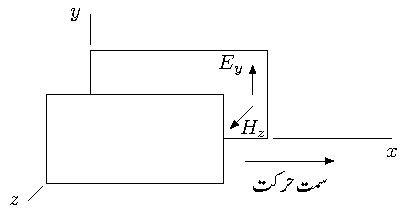
\includegraphics{figWaveguidesInfiniteParallelPlates}
\caption{دو لامحدود وسعت کے متوازی موصل چادروں کا نظام۔}
\label{شکل_مویج_لامحدود_متوازی_چادر}
\end{figure}

ایسی بلند درجی انداز کی بات کرتے ہیں جس میں برقی میدان ہر نقطے پر \عددیء{y} سمتی ہے جبکہ سمت حرکت \عددیء{\ax} ہے۔چونکہ برقی میدان سمت حرکت کے عمودی ہے لہٰذا اس انداز کو \اصطلاح{عرضی برقی انداز}\فرہنگ{عرضی!برقی انداز}\فرہنگ{انداز!عرضی برقی}\حاشیہب{transverse electric mode, TE mode}\فرہنگ{transverse electric mode}\فرہنگ{mode, transverse electric, TE} \تحریر{(TE)} کہا جائے گا۔اگرچہ اس موج میں برقی میدان عرضی ہے، مقناطیسی میدان عرضی اور طولی اجزاء پر مشتمل ہے۔کامل موصل چادروں کی صورت میں چادروں پر برقی میدان صفر ہو گا البتہ چادر سے دور  اس کی کچھ بھی قیمت ممکن ہے۔ایسی عرضی برقی انداز موج کے خصوصیات باآسانی یوں حاصل کئے جا سکتے ہیں کہ اسے دو عرضی برقی و مقناطیسی انداز \تحریر{TEM} امواج کا مجموعہ تصور کیا جائے جو موصل چادروں کے درمیان بار بار انعکاس کرتی ہوں۔

آئیں پہلے شکل \حوالہ{شکل_مویج_دو_عرضی_امواج_خالی_خلاء} پر غور کریں جہاں خالی خلاء میں ایک ہی تعدد کے دو سطحی \تحریر{TEM} امواج کے ملاپ کی صورت حال دکھائی گئی ہے۔اس شکل میں امواج خطی قطبی تصور کئے گئے ہیں جن کا برقی میدان صفحہ کے عمودی فرض کیا گیا ہے۔موج الف کی شعاع اوپر بائیں ہاتھ سے نیچے دائیں ہاتھ کی طرف جبکہ موج ب کی شعاع نیچے بائیں ہاتھ سے اوپر دائیں ہاتھ کی جانب گامزن ہے۔یوں ان کا آپس میں ملاپ کسی زاویے پر ہوتا ہے۔شکل میں گہری سیاہی کی ٹھوس لکیر سے موج کی چوٹی جبکہ ہلکی سیاہی کے ٹھوس لکیر سے اس کا نشیب دکھایا گیا ہے۔یوں سطحی موج الف کی چوٹیاں اور نشیب، شعاع الف کے عمودی دکھائے گئے ہیں۔گہری سیاہی کے ٹھوس لکیر کو برقی میدان کی چوٹی تصور کیا جائے۔یوں اس لکیر پر برقی میدان زیادہ سے زیادہ قیمت رکھتا ہے اور اس کی سمت صفحہ سے عمودی باہر جانب کو ہے۔اسی طرح ہلکی ٹھوس لکیر میدان کی نشیب کو ظاہر کرتی ہے لہٰذا یہاں میدان کی قیمت زیادہ سے زیادہ ہو گی البتہ اس کی سمت صفحہ کے عمودی اندر جانب کو ہو گی۔چوٹی اور نشیب کے درمیان فاصلہ \عددیء{\tfrac{\lambda_0}{2}} کے برابر ہے۔ 
%
\begin{figure}
\centering
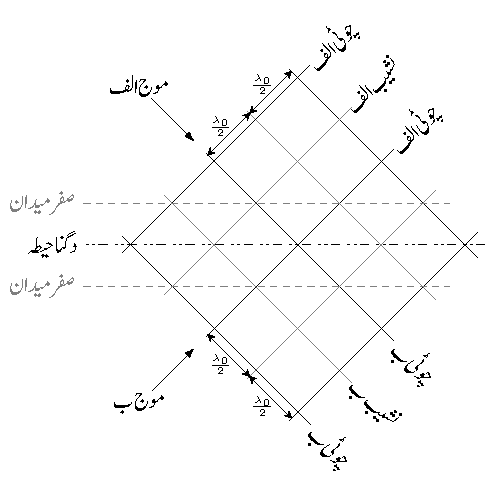
\includegraphics{figWaveguidesTwoIntersectingTEMwaves}
\caption{دو عرضی برقی و مقناطیسی امواج خلاء میں مختلف سمتوں میں حرکت کر رہی ہیں۔}
\label{شکل_مویج_دو_عرضی_امواج_خالی_خلاء}
\end{figure}

جس نقطے پر ایک موج کی چوٹی اور دوسری موج کا نشیب ملتے ہیں اس نقطے پر کل میدان صفر کے برابر ہو گا۔یوں جہاں گہری سیاہی اور ہلکی سیاہی کے لکیر ملتے ہیں وہاں میدان صفر ہو گا۔شکل میں ہلکی سیاہی میں ایسی دو نقطہ دار لکیریں کھینچی گئی ہیں جن پر میدان صفر کے برابر ہے۔آپ غور کر کے تسلی کر لیں کہ ان لکیروں کے ہر نقطے پر برقی میدان صفر ہی ہے۔مزید آپ ذہن میں دونوں امواج کو حرکت دیتے ہوئے تسلی کر لیں کہ امواج کے حرکت کے باوجود ان دو لکیروں پر میدان صفر ہی رہتا ہے۔اسی طرح جن نقطوں پر دونوں امواج کی چوٹیاں آپس میں ملتی ہوں یا دونوں کے نشیب آپس میں ملتے ہوں وہاں میدان دگنا ہو گا۔شکل میں ہلکی سیاہی اور دو نقطوں والی ایسی ایک عدد  لکیر دکھائی گئی ہے جہاں میدان دگنا پایا جائے گا۔

صفر میدان دکھاتے نقطہ دار لکیر پر برقی میدان صفر کے برابر ہے لہٰذا ان پر موصل سطح کے سرحدی برقی میدان کا شرط پورا اترتا ہے۔یوں ان لکیروں پر، صفحہ کے عمودی  موصل چادر رکھے جا سکتے ہیں۔البتہ ایسا کرنے سے موج کی سیدھی حرکت متاثر ہو گی چونکہ آمدی زاویے کے برابر، موصل سطح پر، انعکاسی زاویے سے موج انعکاس کرے گی۔یوں موج موصل سطح سے گزر نہیں پائے گی۔ہاں اگر دو موصل چادروں کے درمیان ان امواج کو بھیجا جائے، تب یہ دونوں موصل سطحوں کے درمیان بار بار انعکاس کرتی حرکت کریں گی۔شکل \حوالہ{شکل_مویج_شعاع_انعکاس_کرتی_حرکت_کرتی_ہے} میں ایسا دکھایا گیا ہے۔ شکل \حوالہ{شکل_مویج_خالی_خلاء_اور_میوج_طول-موج} میں مویج میں موج کی چوٹی اور نشیب دکھائے گئے ہیں۔خالی خلاء میں طول موج اور مویج میں طول موج کا تعلق بھی دکھایا گیا ہے۔ اس شکل میں موصل چادروں کے درمیان میدان ہوبہو شکل \حوالہ{شکل_مویج_دو_عرضی_امواج_خالی_خلاء} میں دو متوازی نقطہ دار لکیروں کے درمیان میدان ہے۔یہاں بھی گہری سیاہی میں ٹھوس لکیر \عددیء{\kvec{E}} کی چوٹی اور ہلکی سیاہی میں لکیر اس کا نشیب ہے۔موصل چادر پر یہ دونوں مل کر صفر برقی میدان پیدا کرتے ہیں۔   

\begin{figure}
\centering
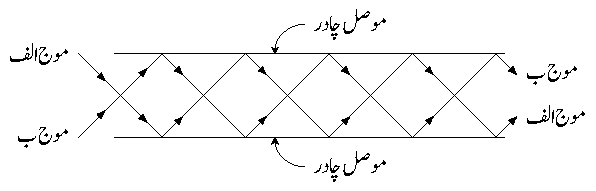
\includegraphics{figWaveguidesTwoConductingSheetsTwoTEMwaves}
\caption{شعاعیں دو چادروں کے درمیان بار بار انعکاس کرتی حرکت کرتی ہیں۔}
\label{شکل_مویج_شعاع_انعکاس_کرتی_حرکت_کرتی_ہے}
\end{figure}
%
\begin{figure}
\centering
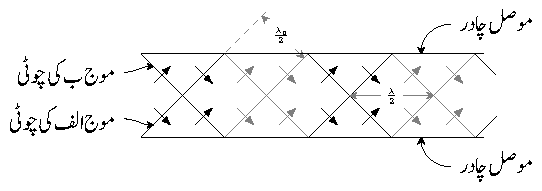
\includegraphics{figWaveguidesTwoConductingSheetsTwoTEMwavesWavefronts}
\caption{موجوں کی چوٹیاں، نشیب، خالی خلاء اور مویج میں طول موج۔}
\label{شکل_مویج_خالی_خلاء_اور_میوج_طول-موج}
\end{figure}

اگرچہ ہم دو عدد عرضی برقی و مقناطیسی \تحریر{TEM} امواج کی بات کرتے آ رہے ہیں، درحقیقت ان کا مجموعہ بلند درجی \تحریر{TE} انداز کی موج ہے۔بلند درجی انداز کے موج کی اہم خصوصیت  یہ ہے کہ اس کا طول موج ایک مخصوص حد سے کم ہونا لازم ہے۔ایسا نہ ہونے کی صورت میں یہ مویج سے نہیں گزر سکتی۔طول کی یہ حد \اصطلاح{انقطاعی طول}\فرہنگ{انقطاعی طول}\فرہنگ{طول!انقطاعی}\حاشیہب{cutoff wavelength}\فرہنگ{cutoff wavelength}\فرہنگ{wavelength!cutoff} پکاری جاتی ہے۔ آئیں انقطاعی طول حاصل کریں۔

 \begin{figure}
\centering
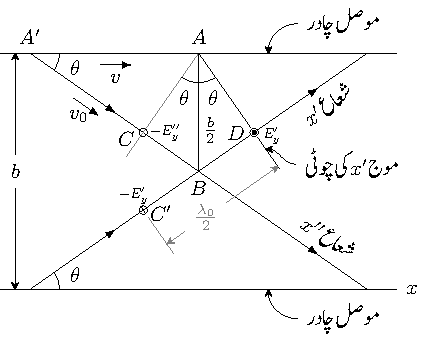
\includegraphics{figWaveguidesTwoConductingSheetsCutoffWavelength}
\caption{متوازی لامحدود وسعت کے چادروں کے مویج میں میدان کے اجزاء۔}
\label{شکل_مویج_متوازی_چادر_مویج_اجزاء_میدان}
\end{figure}

شکل \حوالہ{شکل_مویج_متوازی_چادر_مویج_اجزاء_میدان} میں \تحریر{TE} موج کے دو \تحریر{TEM} اجزاء دکھائے گئے ہیں جو \عددیء{x'} اور \عددیء{x''} سمت میں گامزن ہیں۔دونوں جزو موصل چادر یعنی \عددیء{x} محدد کے ساتھ \عددیء{\theta} زاویہ بناتے ہیں۔برقی میدان صفحہ کے عمودی \عددیء{y} محدد کی سمت میں ہے۔چادروں کے درمیان فاصلہ \عددیء{b} ہے۔نقطہ \عددیء{D} پر موج \عددیء{x'} کی چوٹی ہے لہٰذا یہاں برقی میدان \عددیء{E_y'} مثبت  قیمت رکھتا ہے جو صفحہ کے عمودی باہر کو ہے اور جسے گول دائرے میں بند نقطے سے ظاہر کیا گیا ہے۔ اس نقطے پر لکیر \عددیء{AD} لہر کی چوٹی ظاہر کرتی ہے۔عین اسی لمحہ نقطہ \عددیء{C} پر موج \عددیء{x''} کا نشیب ہے جسے گول دائرے میں بند صلیبی نشان سے ظاہر کیا گیا ہے۔اس لہر کے نشیب کو ہلکی سیاہی میں لکیر \عددیء{AC} سے ظاہر کیا گیا ہے۔ایک لہر کی چوٹی اور دوسرے لہر کا نشیب نقطہ \عددیء{A} پر مل کر صفر میدان پیدا کرتے ہیں۔ہم جانتے ہیں کہ عین دو چادروں کے درمیان دونوں امواج کی چوٹیاں مل کر دگنا میدان پیدا کرتی ہیں۔اس نقطے کو شکل میں \عددیء{B} سے ظاہر کیا گیا ہے۔یوں موج \عددیء{x''} کا نشیب \عددیء{C} پر جبکہ اس کی چوٹی \عددیء{B} پر ہے۔اس طرح ان نقطوں کے درمیان فاصلہ طول موج کا چوتھا حصہ ہو گا۔اسی طرح \عددیء{BD} اور \عددیء{C'B} بھی طول موج کے چوتھائی برابر  ہیں
\begin{align}
BC=BC'=BD=\frac{\lambda_0}{4}
\end{align}
جہاں لامحدود خلاء میں \تحریر{TEM} موج کا طول موج \عددیء{\lambda_0} ہے اور یہ خلاء اسی مادے سے بھری ہے جو دو چادروں کے درمیان پایا جاتا ہے۔موصل چادر پر ایک موج کی کوئی بھی چوٹی اور دوسری موج کا کوئی بھی نشیب مل کر صفر میدان پیدا کر سکتے ہیں۔یوں مندرجہ بالا مساوات کی عمومی شکل
\begin{align}\label{مساوات_مویج_چوٹی_نشیب_ختم_عمومی}
BC=\frac{n \lambda_0}{4}
\end{align}
ہے جہاں \عددیء{n=1,2,3,\cdots} ہو سکتے ہیں۔جفت \عددیء{n} کی صورت میں دو چادروں کے عین درمیان برقی میدان صفر حاصل ہو گا جبکہ طاق \عددیء{n} کی صورت میں یہاں میدان دگنا ہو گا۔ان حقائق ہر تفصیلاً جلد بات کی جائے گی۔شکل \حوالہ{شکل_مویج_متوازی_چادر_مویج_اجزاء_میدان} میں تکون \عددیء{ABC} سے
\begin{align*}
AB \sin \theta = \frac{b}{2}\sin \theta =\frac{n \lambda_0}{4}
\end{align*}
یعنی
\begin{align}\label{مساوات_مویج_طول_اور_درجہ_انداز}
\lambda_0 = \frac{2b}{n} \sin \theta
\end{align}
لکھا جا سکتا ہے جہاں لمبائی \عددیء{BC} کے لئے مساوات \حوالہ{مساوات_مویج_چوٹی_نشیب_ختم_عمومی} استعمال کیا گیا۔اس مساوات کے تحت زیادہ سے زیادہ طول موج \عددیء{\lambda_{0c}} کی قیمت \عددیء{\sin \theta=1} یعنی \عددیء{\theta=90^{\circ}} پر
\begin{align}\label{مساوات_مویج_طول_موج_بالمقابل_درجہ_موج}
\lambda_{0c}=\frac{2b}{n}
\end{align}
 حاصل ہوتی ہے جس سے \عددیء{n} کی ہر قیمت کے مقابل طول کی انقطاعی قیمت حاصل کی جا سکتی ہے۔جب \عددیء{n=1} ہو تب
 \begin{align}\label{مساوات_مویج_دو_چادر_انقطاعی_طول_موج}
\lambda_{0c}=2b
\end{align}
حاصل ہوتا ہے۔یہ کم تر درجے کی \تحریر{TE} موج کا انقطاعی طول ہے جو ان چادروں کے درمیان صفر کر سکتی ہے۔یہ مساوات کہتا ہے کہ چادروں کے درمیان فاصلہ کم از کم آدھے طول کے برابر ہو گا تو موج چادروں کے درمیان سے گزر پائے گی۔

\عددیء{n=1} کو بلند درجی \تحریر{TE} امواج کا کم تر درجہ کہا جاتا ہے۔\عددیء{n=2} اس سے ایک قدم بلند  درجے کی موج کہلائے گی اور اس کا انقطاعی طول
\begin{align}
\lambda_{0c}=b
\end{align}
ہو گا۔یوں \عددیء{n=2} درجے کی \تحریر{TE} موج کے گزرنے کا لئے چادروں کے درمیان کم از کم فاصل موج کے طول کے برابر ضروری ہے۔اسی طرح \عددیء{n=3} کے لئے \عددیء{\lambda_{0c}=\tfrac{2b}{3}} حاصل ہوتا ہے، وغیرہ وغیرہ۔

مساوات \حوالہ{مساوات_مویج_طول_موج_بالمقابل_درجہ_موج} اور مساوات \حوالہ{مساوات_مویج_طول_اور_درجہ_انداز} کو ملا کر
\begin{align}
\lambda_0=\lambda_{0c} \sin \theta
\end{align}
یا
\begin{align}
\theta=\sin^{-1}\frac{\lambda_0}{\lambda_{0c}}
\end{align}
لکھا جا سکتا ہے۔یوں کسی بھی درجے کی موج کا انقطاعی زاویہ \عددیء{\theta=90^{\circ}} حاصل ہوتا ہے۔اس زاویے پر موج  دونوں چادروں کے مابین، \عددیء{x} تبدیل کئے بغیر،  انعکاس کرتی رہتی ہے۔یوں چادروں کے درمیان ساکن موج پیدا ہوتی ہے جو \عددیء{x} سمت میں طاقت منتقل نہیں کر سکتی۔اگر طول موج \عددیء{\lambda_0} انقطاعی طول موج \عددیء{\lambda_{0c}} سے قدر کم ہو تب \عددیء{\theta} کی قیمت \عددیء{90^{\circ}} سے کم ہو گی اور موج، بار بار انعکاس کرتی ہوئی، چادروں کے درمیان \عددیء{x} سمت میں حرکت کر پائے گی۔جیسے شکل \حوالہ{شکل_مویج_طول_موج_اور_زاویہ_انعاکس} میں دکھایا گیا ہے، طول موج مزید کم کرنے سے زاویہ مزید کم ہوتا ہے۔آخر کار انتہائی کم طول موج پر صورت حال لامحدود خلاء میں موج کے حرکت مانند ہو جاتی ہے اور یہ شعاع کی طرح چادروں کے درمیان سیدھا گزرنے کے قابل ہو جاتی ہے۔

\begin{figure}
\centering
\begin{subfigure}{0.4\textwidth}
\centering
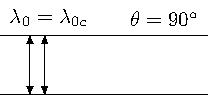
\includegraphics{figWaveguidesTwoConducorsAngleNinty}
\caption{طول موج، عین انقطاعی طول موج کے برابر ہے۔}
\end{subfigure}%
%
\begin{subfigure}{0.4\textwidth}
\centering
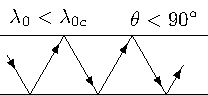
\includegraphics{figWaveguidesTwoConducorsAngleAbitLessThanNinty}
\caption{طول موج، انقطاعی طول موج سے قدر کم ہے۔}
\end{subfigure}%

\begin{subfigure}{0.4\textwidth}
\centering
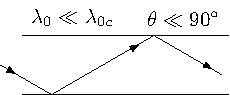
\includegraphics{figWaveguidesTwoConducorsAngleMuchLessThanNinty}
\caption{طول موج مزید کم کرنے سے زاویہ بھی مزید کم ہوتا ہے۔}
\end{subfigure}%
\begin{subfigure}{0.4\textwidth}
\centering
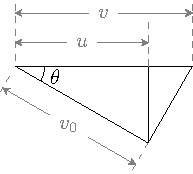
\includegraphics{figWaveguidesTwoConducorsPhaseGroupVelocities}
\caption{مختلف اقسام کے رفتار کا تعلق۔}
\end{subfigure}%
\caption{طول موج اور انعکاس موج کے زاویے۔ مختلف اقسام کے رفتاروں کا آپس میں تعلق۔}
\label{شکل_مویج_طول_موج_اور_زاویہ_انعاکس}
\end{figure}

شکل \حوالہ{شکل_مویج_متوازی_چادر_مویج_اجزاء_میدان} میں \تحریر{TEM} امواج کی \اصطلاح{دوری رفتار}\فرہنگ{دوری!رفتار}\فرہنگ{رفتار!دوری}\حاشیہب{phase velocity}\فرہنگ{phase velocity} \عددیء{v_0} لامحدود خلاء میں آزاد موج کی دوری رفتار
\begin{align}
v_0=\frac{1}{\sqrt{\mu \epsilon}} \quad (\si{\meter \per \second})
\end{align}
ہی ہے جہاں خلاء کا مقناطیسی مستقل \عددیء{\mu} اور اس کا برقی مستقل \عددیء{\epsilon} ہیں۔شکل \حوالہ{شکل_مویج_طول_موج_اور_زاویہ_انعاکس}-د میں \تحریر{TE} موج کی \عددیء{x} سمت میں دوری رفتار \عددیء{v} ہے۔\تحریر{TE} موج کی چوٹی یا نشیب یا کوئی اور زاویائی نقطہ اس رفتار سے \عددیء{x} سمت میں حرکت کرتا نظر آئے گا۔ان دو اقسام کے رفتار کا تعلق شکل \حوالہ{شکل_مویج_طول_موج_اور_زاویہ_انعاکس}-د سے
\begin{align}
\frac{v_0}{v}=\cos \theta
\end{align}
لکھا جا سکتا ہے جس سے
\begin{align}\label{مساوات_مویج_دوری_رفتار_تعلق_الف}
v=\frac{v_0}{\cos \theta}=\frac{1}{\sqrt{\mu \epsilon} \cos \theta} \quad \quad \si{\meter\per\second}
\end{align}
حاصل ہوتا ہے۔اس مساوات کے تحت جیسے جیسے طول موج کو انقطاعی طول موج کے قریب لایا جائے، ویسے ویسے \تحریر{TE} موج کی دوری رفتار کی قیمت بڑھتی ہے حتٰی کہ عین \عددیء{\lambda_{0c}} پر دوری رفتار لامحدود قیمت اختیار کر لیتی ہے۔اس کے برعکس جیسے جیسے طول موج کو کم کیا جائے، یعنی جیسے جیسے \عددیء{\theta} کو کم کیا جائے، ویسے ویسے \تحریر{TE} موج کی دوری رفتار \تحریر{TEM} کے دوری رفتار کے قریب ہو گی حتٰی کہ انتہائی کم طول موج یعنی انتہائی بلند تعدد کے موج کی صورت میں یہ قیمت \عددیء{v_0} کے برابر ہو جائے گی۔ یوں مویج میں بند، بلند درجی موج کا دوری رفتار \تحریر{TEM} موج کے دوری رفتار سے زیادہ یا اس کے برابر ممکن ہے۔طاقت کی منتقلی انعکاس کرتی موج کے \اصطلاح{مجموعی رفتار}\فرہنگ{مجموعی رفتار}\فرہنگ{رفتار!مجموعی}\حاشیہب{group velocity}\فرہنگ{group velocity} سے ہوتی ہے جسے شکل میں \عددیء{u} سے ظاہر کیا گیا ہے۔شکل \حوالہ{شکل_مویج_طول_موج_اور_زاویہ_انعاکس}-د سے
\begin{align}\label{مساوات_مویج_دوری_رفتار_تعلق_ب}
u=v_0 \cos \theta
\end{align}
لکھا جا سکتا ہے لہٰذا طاقت کی منتقلی کی رفتار \تحریر{TEM} کے رفتار سے کم یا اس کے برابر ممکن ہے۔طاقت کسی صورت بھی \تحریر{TEM} موج کی رفتار سے زیادہ رفتار پر منتقل کرنا ممکن نہیں ہے۔یہ حقیقت آئن سٹائن کے قانون کے عین مطابق ہے جس کے تحت کوئی بھی چیز رفتار شعاع سے تجاوز نہیں کر سکتی۔یاد رہے کہ \تحریر{TE} موج کی دوری رفتار درحقیقت کسی چیز کی منتقلی نہیں کرتی لہٰذا اس کی قیمت \عددیء{v_0} سے بڑھ سکتی ہے۔مساوات \حوالہ{مساوات_مویج_دوری_رفتار_تعلق_الف} اور مساوات \حوالہ{مساوات_مویج_دوری_رفتار_تعلق_ب}  کو ملا کر 
\begin{align}\label{مساوات_مویج_دوری_رفتار_تعلق_پ}
u v =v_0^2
\end{align}
حاصل ہوتا ہے۔

دو چادروں میں بند ہونے سے \تحریر{TEM} موج کا تعدد تبدیل نہیں ہوتا۔اسی طرح ایسے دو یکساں تعدد کے امواج سے حاصل \تحریر{TE} موج کا تعدد بھی وہی رہتا ہے۔چونکہ طول موج ضرب تعدد کا حاصل رفتار کے برابر ہوتا ہے لہٰذا مساوات \حوالہ{مساوات_مویج_دوری_رفتار_تعلق_الف} کو
\begin{align*}
f \lambda=\frac{f \lambda_0}{\cos \theta}
\end{align*}
لکھا جا سکتا ہے جس سے
\begin{align*}
\lambda=\frac{\lambda_0}{\cos \theta}
\end{align*}
حاصل ہوتا ہے جو بلند درجہ موج کے طول \عددیء{\lambda} اور آزاد موج کے طول \عددیء{\lambda_0} کا تعلق ہے۔

\begin{figure}
\centering
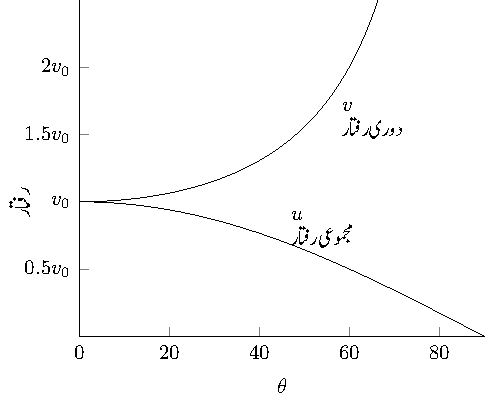
\includegraphics{figWaveguidesTwoConducorsPhaseGroupVelocitiesGraphicalView}
\caption{دوری اور مجموعی رفتار بالمقابل زاویہ موج۔}
\label{شکل_مویج_دوری_مجموعی_رفتار_بالمقابل_زاویہ}
\end{figure} 

شکل \حوالہ{شکل_مویج_دوری_مجموعی_رفتار_بالمقابل_زاویہ} میں دوری رفتار بالمقابل زاویہ موج اور مجموعی رفتار بالمقابل زاویہ موج دکھائے گئے ہیں۔جیسے جیسے \عددیء{\theta} کی قیمت \عددیء{90^{\circ}} کے قریب آتی ہے ویسے ویسے دوری رفتار کی قیمت لامحدود جبکہ مجموعی رفتار کی قیمت صفر کے قریب تر ہوتی ہے۔

حقیقت میں دو متوازی لامحدود وسعت\حاشیہد{حقیقی دنیا میں لا محدود وسعت کے چادر نہیں پائے جاتے۔} کے چادروں پر مبنی مویج کہیں نہیں پایا جاتا۔حقیقی مویج عموماً کھوکھلے مستطیل یا کھوکھلے نالی کے اشکال رکھتے ہیں۔چونکہ برقی میدان کے عمودی موصل چادر رکھنے سے میدان متاثر نہیں ہوتا لہٰذا دو لامحدود وسعت کے متوازی چادر، جن کے درمیان فاصلہ \عددیء{b} ہو، میں \تحریر{TE} موج کے عمودی دو چادر رکھنے سے  میدان میں کوئی تبدیلی رونما نہیں ہو گی، لیکن ایسا کرنے سے مستطیل مویج حاصل ہوتا ہے۔شکل \حوالہ{شکل_مویج_مستطیل}-الف میں مستطیلی مویج بنتا  دکھایا گیا ہے جہاں \عددیء{d} فاصلے پر دو متوازی چادر رکھے گئے ہیں۔مستطیل شکل کے علاوہ بقایا چادر ہٹانے سے مستطیل مویج حاصل ہوتا ہے جسے شکل \حوالہ{شکل_مویج_مستطیل}-ب میں دکھایا گیا ہے۔اس طرح ہم دیکھتے ہیں کہ اگرچہ دو لامحدود چادروں کا مویج تو استعمال نہیں ہوتا لیکن اس کے \تحریر{TE} امواج جوں کے توں مستطیل مویج کے لئے استعمال کئے جا سکتے ہیں۔موجودہ \تحریر{TE} امواج کے نقطہ نظر سے مستطیل کی \عددیء{d} لمبائی کچھ بھی ممکن ہے۔

\begin{figure}
\centering
\begin{subfigure}{0.4\textwidth}
\centering
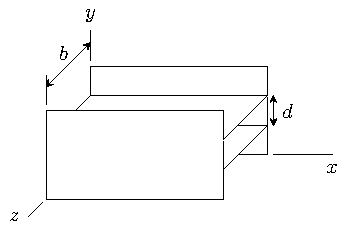
\includegraphics{figWaveguidesInfiniteParallelPlatesToRectangularWaveguide}
\caption{لامحدود متوازی چادر مویج سے مستطیلی مویج کا حصول۔}
\label{شکل_مویج_حصول_مستطیل}
\end{subfigure}%
%
\begin{subfigure}{0.4\textwidth}
\centering
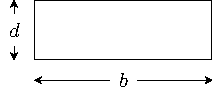
\includegraphics{figWaveguidesRectangularWaveguide}
\caption{مستطیلی مویج کا رقبہ عمودی تراش۔}
\label{شکل_مویج_رقبہ_عمودی_تراش_مستطیل}
\end{subfigure}
\caption{مستطیلی مویج کا حصول اور اس کا رقبہ عمودی تراش۔}
\label{شکل_مویج_مستطیل}
\end{figure}

لامحدود چادر کے مویج پر غور کرنے سے انقطاعی طول موج کے علاوہ دوری رفتار اور مجموعی رفتار کے مساوات بھی حاصل کئے گئے۔دیگر بلند درجے کے امواج پر معلومات حاصل کرنے کی خاطر میکس ویل کے مساوات حل کرنا لازم ہے۔آئیں  مستطیل مویج کے لئے میکس ویل مساوات حل کرتے ہیں۔

\حصہ{کھوکھلا مستطیلی مویج} 
مستطیل مویج کے اطراف پر برقی اور مقناطیسی سرحدی شرائط، کارتیسی محدد میں نہایت آسانی سے لاگو کئے جا سکتے ہیں۔اسی لئے مستطیلی مویج کو کارتیسی نظام میں حل کیا جائے گا۔ہم کارتیسی نظام میں میکس ویل کے مساوات سے  موج کی مساوات حاصل کرتے ہیں۔مویج کو \عددیء{x} محدد پر رکھتے ہوئے ہم سمت موج کو اسی سمت حرکت کے پابند بناتے ہیں اور ساتھ ہی ساتھ اسے سائن نما تصور کرتے ہیں۔اس کے بعد بلند درجے موج کی قسم کا انتخاب کرتے ہیں۔یوں ہم برقی میدان \عددیء{E} کو سمت موج کے عمودی رہنے کے پابند رکھتے ہوئے \اصطلاح{عرضی برقی}\فرہنگ{عرضی!برقی}\حاشیہب{transverse electric, TE}\فرہنگ{transverse electric, TE} \تحریر{TE} موج پر غور کر سکتے ہیں یا مقناطیسی میدان کو سمت موج کے عمودی رہنے کے پابند رکھتے ہوئے \اصطلاح{عرضی مقناطیسی}\حاشیہب{transverse magnetic, TM} \تحریر{TM} موج پر غور کر سکتے ہیں۔\تحریر{TEM} موج میں برقی اور مقناطیسی میدان سمت حرکت کے عمودی ہوتے ہیں۔بلند درجی موج میں میدان، سمت حرکت کی سمت میں بھی پائے جاتے ہیں۔اب عرضی برقی \تحریر{TE} موج کی صورت میں \عددیء{E_x=0} ہو گا لہٰذا ایسی صورت میں \عددیء{H_x} صفر کے برابر نہیں ہو سکتا۔اگر \عددیء{H_x} بھی صفر کے برابر ہو تب موج \تحریر{TEM} قسم کی ہو گی نا کہ \تحریر{TE} قسم کی۔\تحریر{TE} کی صورت میں تمام مساوات کو \عددیء{H_x} کی صورت میں لکھنا بہتر ثابت ہوتا ہے۔حاصل موج پر سرحدی شرائط لاگو کرتے ہوئے اسے \عددیء{H_x} کے لئے حل کیا جاتا ہے۔حاصل \عددی{H_x} کو بقایا مساوات میں پر کرتے ہوئے \عددیء{E_y}، \عددیء{E_z}، \عددیء{H_y} اور \عددیء{H_z} حاصل کئے جاتے ہیں۔یوں برقی اور مقناطیسی میدان کے تمام کارتیسی اجزاء کی مکمل معلومات حاصل ہوتی ہے۔یہ عمومی طریقہ کار ہے جسے دیگر مسائل حل کرنے کے لئے بھی استعمال کیا جا سکتا ہے۔

اس طریقے کو مستطیلی مویج میں \تحریر{TE} موج کے لئے تفصلیلاً  استعمال کرتے ہیں۔ایسا کرنے کی خاطر مندرجہ ذیل قدم سلسلہ وار اٹھائے جائیں گے۔
\begin{itemize}\label{اقدام_مویج_آٹھ_قدم}
\item
میکس ویل مساوات سے شروع کریں۔
\item
موج کو وقت کے ساتھ سائن نما رہنے کا پابند بنائیں۔
\item
موج کو \عددیء{x} سمت کے ساتھ سائن نما رہنے کا پابند بناتے ہوئے  حرکی مستقل بروئے کار لائیں۔
\item
بلند درجی موج کا انتخاب کریں۔ہم \تحریر{TE} موج کا انتخاب کرتے ہوئے \عددیء{E_x=0} اور \عددیء{H_x \ne 0} رکھیں گے۔
\item
بقایا چار اجزاء یعنی \عددیء{E_y}، \عددیء{E_z}، \عددیء{H_y} اور \عددیء{H_z} کے مساوات \عددیء{H_x} کی صورت میں لکھیں۔
\item
موج کی مساوات \عددیء{H_x} کی صورت میں حاصل کریں۔
\item
مستطیلی مویج کے اطراف کے سرحدی شرائط لاگو کرتے ہوئے موج کی اس مساوات کو \عددیء{H_x} کے لئے حل کریں۔
\item
\عددیء{E_y}، \عددیء{E_z}، \عددیء{H_y} اور \عددیء{H_z} کے مساوات میں حاصل \عددیء{H_x} پر کرتے ہوئے ان کی مساوات بھی حاصل کریں۔
\end{itemize}  

ان اقدامات سے مکمل حل حاصل ہو گا۔

آئیں پہلے قدم سے شروع کرتے ہوئے میکس ویل کے مساوات کو کارتیسی نظام میں لکھتے ہیں۔صفحہ \حوالہصفحہ{مساوات-میکس_ویل_تفرقی_الف} پر مساوات \حوالہ{مساوات-میکس_ویل_تفرقی_الف} اور  مساوت \حوالہ{مساوات-میکس_ویل_تفرقی_ب}
\begin{align*}
\nabla \times \kvec{E}&=-\frac{\partial \kvec{B}}{\partial t}\\
\nabla \times \kvec{H}&=\kvec{J}+\frac{\partial \kvec{D}}{\partial t}
\end{align*}
کارتیسی محدد میں
\begin{align}
\frac{\partial E_z}{\partial y}-\frac{\partial E_y}{\partial z}+\mu \frac{\partial H_x}{\partial t}&=0  \label{مساوات_مویج_میکس_ویل_الف}\\
\frac{\partial E_x}{\partial z}-\frac{\partial E_z}{\partial x}+\mu \frac{\partial H_y}{\partial t}&=0   \label{مساوات_مویج_میکس_ویل_ب}\\
\frac{\partial E_y}{\partial x}-\frac{\partial E_x}{\partial y}+\mu \frac{\partial H_z}{\partial t}&=0 \label{مساوات_مویج_میکس_ویل_پ}
\end{align}
اور
\begin{align}
\frac{\partial H_z}{\partial y}-\frac{\partial H_y}{\partial z}-\sigma E_x-\epsilon \frac{\partial E_x}{\partial t}&=0  \label{مساوات_مویج_میکس_ویل_ت}\\
\frac{\partial H_x}{\partial z}-\frac{\partial H_z}{\partial x}-\sigma E_y-\epsilon \frac{\partial E_y}{\partial t}&=0  \label{مساوات_مویج_میکس_ویل_ٹ}\\
\frac{\partial H_y}{\partial x}-\frac{\partial H_x}{\partial y}-\sigma E_z-\epsilon \frac{\partial E_z}{\partial t}&=0 \label{مساوات_مویج_میکس_ویل_ث}
\end{align}
لکھے جائیں گے جہاں \عددیء{\kvec{B}=\mu \kvec{H}} اور \عددیء{\kvec{D}=\epsilon \kvec{E}} کا استعمال کیا گیا ہے۔اسی طرح خالی خلاء میں \عددیء{\rho_h=0} لیتے ہوئے  مساوات \حوالہ{مساوات_میکس_ویل_گاوس_قانون_نقطہ} اور مساوات \حوالہ{مساوات_میکس_ویل_مقناطیسی_میدان_دو_قطب} کارتیسی محدد میں
\begin{align}
\frac{\partial E_x}{\partial x}+\frac{\partial E_y}{\partial y}+\frac{\partial E_z}{\partial z}&=0 \label{مساوات_مویج_میکس_ویل_ج}\\
\frac{\partial H_x}{\partial x}+\frac{\partial H_y}{\partial y}+\frac{\partial H_z}{\partial z}&=0 \label{مساوات_مویج_میکس_ویل_چ}
\end{align}
لکھے جائیں گے۔

اب دوسرا قدم کہتا ہے کہ موج وقت کے ساتھ سائن نما تعلق رکھتا ہے جبکہ تیسرا قدم کہتا ہے کہ موج \عددیء{x} فاصلے کے ساتھ بھی سائن نما تعلق رکھتا ہے۔ساتھ ہی ساتھ \عددیء{x} سمت میں حرکی مستقل بھی بروئے کار لانا ہے۔ان دو اقدام کو استعمال کرتے ہوئے میدان کے تمام اجزاء لکھتے ہیں۔یوں \عددیء{E_y} اور \عددیء{H_x} کو مثال بناتے ہوئے
\begin{gather}
\begin{aligned}\label{مساوات_مویج_سائن_نما_کی_قید}
E_y&=E_1 e^{j \omega t -\gamma x} \\
H_x&=H_1 e^{j \omega t -\gamma x}
\end{aligned}
\end{gather}
لکھے جائیں گے جہاں
\begin{align*}
\gamma&=\text{\RL{حرکی مستقل}}=\alpha+j \beta \\
\alpha&=\text{\RL{تقلیلی مستقل}}\\
\beta&=\text{\RL{زاویائی مستقل}}
\end{align*}
ہیں۔مساوات \حوالہ{مساوات_مویج_سائن_نما_کی_قید} کے طرز پر بقایا میدان بھی لکھتے ہوئے مساوات \حوالہ{مساوات_مویج_میکس_ویل_الف}
\begin{align*}
\left[\frac{\partial E_z}{\partial y}-\frac{\partial E_y}{\partial z}+j \omega \mu H_x\right] e^{j \omega t -\gamma z}&=0  
\end{align*}
یا
\begin{align}
\frac{\partial E_z}{\partial y}-\frac{\partial E_y}{\partial z}+j \omega \mu H_x&=0  
\end{align}
لکھا جائے۔اسی طرح مساوات \حوالہ{مساوات_مویج_سائن_نما_کی_قید} کے طرز پر بقایا میدان بھی لکھتے ہوئے مساوات \حوالہ{مساوات_مویج_میکس_ویل_ب}  تا مساوات \حوالہ{مساوات_مویج_میکس_ویل_چ} یوں لکھے جائیں گے۔
\begin{align}
\frac{\partial E_x}{\partial z}+\gamma E_z+j \omega \mu H_y&=0  \\
-\gamma E_y-\frac{\partial E_x}{\partial y}+j \omega \mu H_z&=0
\end{align}
%
\begin{align}
\frac{\partial H_z}{\partial y}-\frac{\partial H_y}{\partial z}-(\sigma+j \omega \epsilon)E_x&=0 \\
\frac{\partial H_x}{\partial z}+\gamma H_z-(\sigma+j \omega \epsilon)E_y&=0  \\
-\gamma H_y-\frac{\partial H_x}{\partial y}-(\sigma+j \omega \epsilon)E_z&=0 
\end{align}
%
\begin{align}
-\gamma E_x+\frac{\partial E_y}{\partial y}+\frac{\partial E_z}{\partial z}&=0 \\
-\gamma H_x+\frac{\partial H_y}{\partial y}+\frac{\partial H_z}{\partial z}&=0
\end{align}
مندرجہ بالا آٹھ مساوات میں ترسیلی تار کے برقی رکاوٹ \عددیء{Z} اور برقی فراوانی \عددیء{Y} کی طرز کے مستقل
\begin{align}\label{مساوت_مویج_رکاوٹ_فراوانی}
Z&=-j \omega \mu  \quad \quad \left(\si{\ohm / \meter} \right) \\
Y&=\sigma +j \omega \epsilon \quad \quad \left(\si{\siemens / \meter} \right)
\end{align}
استعمال کرتے ہوئے انہیں قدر چھوٹا لکھتے ہیں۔
\begin{align}
\frac{\partial E_z}{\partial y}-\frac{\partial E_y}{\partial z}-Z H_x&=0  \\
\frac{\partial E_x}{\partial z}+\gamma E_z-Z H_y&=0  \\
-\gamma E_y-\frac{\partial E_x}{\partial y}-Z H_z&=0
\end{align}
%
\begin{align}
\frac{\partial H_z}{\partial y}-\frac{\partial H_y}{\partial z}-YE_x&=0 \\
\frac{\partial H_x}{\partial z}+\gamma H_z-YE_y&=0  \\
-\gamma H_y-\frac{\partial H_x}{\partial y}-YE_z&=0 
\end{align}
%
\begin{align}
-\gamma E_x+\frac{\partial E_y}{\partial y}+\frac{\partial E_z}{\partial z}&=0 \\
-\gamma H_x+\frac{\partial H_y}{\partial y}+\frac{\partial H_z}{\partial z}&=0
\end{align}
 یہ \عددیء{x} سمت میں حرکت کرتی موج کی عمومی مساوات ہیں۔

ابھی تک نا تو مویج کی شکل اور نا ہی بلند درجی موج  کا انتخاب کیا گیا ہے لہٰذا چوتھے قدم کا اطلاق کرتے ہوئے \تحریر{TE} قسم کا انتخاب کرتے ہیں جس کا مطلب ہے کہ \عددیء{E_x=0} لیا جائے گا۔ایسا کرنے سے مندرجہ بالا مساوات   
\begin{align}
\frac{\partial E_z}{\partial y}-\frac{\partial E_y}{\partial z}-Z H_x&=0  \label{مساوات_میوج_الف}\\
\gamma E_z-Z H_y&=0  \label{مساوات_میوج_ب}\\
-\gamma E_y-Z H_z&=0\label{مساوات_میوج_پ}
\end{align}
%
\begin{align}
\frac{\partial H_z}{\partial y}-\frac{\partial H_y}{\partial z}&=0 \label{مساوات_میوج_ت}\\
\frac{\partial H_x}{\partial z}+\gamma H_z-YE_y&=0  \label{مساوات_میوج_ٹ}\\
-\gamma H_y-\frac{\partial H_x}{\partial y}-YE_z&=0 \label{مساوات_میوج_ث}
\end{align}
%
\begin{align}
\frac{\partial E_y}{\partial y}+\frac{\partial E_z}{\partial z}&=0 \label{مساوات_میوج_ج}\\
-\gamma H_x+\frac{\partial H_y}{\partial y}+\frac{\partial H_z}{\partial z}&=0\label{مساوات_میوج_چ}
\end{align}
صورت اختیار کر لیتے ہیں۔

پانچویں قدم پر تمام مساوات کو \عددیء{H_x} کی صورت میں لکھنا ہو گا۔ایسا کرنے کی خاطر پہلے مساوات \حوالہ{مساوات_میوج_ب} اور \حوالہ{مساوات_میوج_پ} سے
\begin{align}\label{مساوات_میوج_ح}
\frac{E_z}{H_y}=-\frac{E_y}{H_z}=\frac{Z}{\gamma}
\end{align}
لکھتے ہیں۔اب \عددیء{\tfrac{E_z}{H_y}} یا \عددیء{\tfrac{E_y}{H_z}} کی شرح قدرتی رکاوٹ کی مانند ہے۔چونکہ  مساوات \حوالہ{مساوات_میوج_ح} میں صرف عرضی اجزاء پائے جاتے ہیں لہٰذا اس شرح کو \اصطلاح{عرضی-موج کی قدرتی رکاوٹ}\فرہنگ{عرضی-موج!قدرتی رکاوٹ}\فرہنگ{قدرتی رکاوٹ!عرضی موج}\حاشیہب{transverse-wave impedance}\فرہنگ{impedance!transverse-wave}\فرہنگ{transverse!wave impedance} \عددیء{Z_{yz}} کہا جائے گا جہاں
\begin{align}\label{مساوات_میوج_خ}
Z_{yz}=\frac{E_y}{H_z}=-\frac{E_z}{H_y}=-\frac{Z}{\gamma}=\frac{j\omega \mu}{\gamma}  \quad \quad (\si{\ohm})
\end{align}
کے برابر ہے۔مساوات \حوالہ{مساوات_میوج_خ} کو مساوات \حوالہ{مساوات_میوج_ث} میں پر کرتے ہوئے \عددیء{H_y} کے لئے حل کرنے سے
\begin{align}\label{مساوات_میوج_د}
H_y=\frac{-1}{\gamma-Y Z_{yz}} \frac{\partial H_x}{\partial y}
\end{align}
حاصل ہوتا ہے۔اسی طرح  مساوات \حوالہ{مساوات_میوج_خ} کو مساوات \حوالہ{مساوات_میوج_ٹ} میں پر کرتے ہوئے \عددیء{H_z} کے لئے حل کرنے سے
\begin{align}\label{مساوات_میوج_ڈ}
H_z=\frac{-1}{\gamma-Y Z_{yz}} \frac{\partial H_x}{\partial z}
\end{align}
حاصل ہوتا ہے۔اب مساوات \حوالہ{مساوات_میوج_د} کو مساوات \حوالہ{مساوات_میوج_خ} میں پر کرتے ہوئے
\begin{align}\label{مساوات_میوج_ذ}
E_z=\frac{Z_{yz}}{\gamma-Y Z_{yz}}\frac{\partial H_x}{\partial y}
\end{align}
اور مساوات \حوالہ{مساوات_میوج_ڈ} کو مساوات \حوالہ{مساوات_میوج_خ} میں پر کرتے ہوئے
\begin{align}\label{مساوات_میوج_ر}
E_y=\frac{-Z_{yz}}{\gamma-Y Z_{yz}}\frac{\partial H_x}{\partial z}
\end{align}
حاصل ہوتے ہیں۔ مساوات \حوالہ{مساوات_میوج_د} تا مساوات \حوالہ{مساوات_میوج_ر} تمام اجزاء کو \عددیء{H_x} کی صورت میں پیش کرتے ہیں۔ 

چھٹے قدم پر ان مساوات سے موج کی مساوات کا حصول ہے۔ایسا کرنے کی خاطر مساوات \حوالہ{مساوات_میوج_د} کا \عددیء{y} کے ساتھ تفرق اور مساوات \حوالہ{مساوات_میوج_ڈ} کا \عددیء{z} کے ساتھ تفرق لیتے ہوئے دونوں حاصل جواب کو مساوات \حوالہ{مساوات_میوج_چ} میں پر کرتے ہوئے
\begin{align*}
-\gamma H_x-\frac{1}{\gamma -Y Z_{yz}} \left(\frac{\partial^2 H_x}{\partial y^2}+\frac{\partial^2 H_x}{\partial z^2} \right)=0
\end{align*}
یا
\begin{align*}
\frac{\partial^2 H_x}{\partial y^2}+\frac{\partial^2 H_x}{\partial z^2}+\gamma \left(\gamma-Y Z_{yz} \right)H_x =0
\end{align*}
حاصل کرتے ہیں جس میں
\begin{align}\label{مساوات_میوج_ڑ}
k^2=\gamma \left(\gamma-Y Z_{yz}\right)
\end{align}
پر کرتے ہوئے
\begin{align}\label{مساوات_میوج_ز}
\frac{\partial^2 H_x}{\partial y^2}+\frac{\partial^2 H_x}{\partial z^2}+k^2 H_x =0
\end{align}
لکھا جا سکتا ہے۔مساوات \حوالہ{مساوات_میوج_ز} مویج کے عرضی برقی موج کی عمومی مساوات ہے۔مویج کا عمودی تراش کسی بھی شکل کا ہو سکتا ہے۔ یہاں چھٹا قدم پورا ہوتا ہے۔

\begin{figure}
\centering
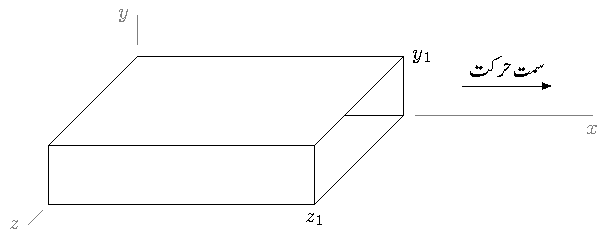
\includegraphics{figWaveguidesRectangularWaveguideThreeD}
\caption{مستطیل مویج۔}
\label{شکل_مویج_مستطیل_مویج_اطراف}
\end{figure}
ساتویں قدم میں مویج کے اطراف کے سرحدی شرائط لاگو کرتے ہوئے موج کو حل کرنا ہے۔شکل \حوالہ{شکل_مویج_مستطیل_مویج_اطراف} میں کامل موصل چادروں سے بنایا گیا مستطیلی مویج دکھایا گیا ہے جس کی چوڑائی \عددیء{z_1} اور اونچائی \عددیء{y_1} ہے۔موصل اور ہوا کے سرحدی برقی شرائط کے مطابق سرحد پر متوازی برقی میدان صفر ہوتا ہے لہٰذا مویج کے اطراف پر متوازی \عددیء{E} صفر ہو گا۔یوں مویج کے نچلی اور  بالائی سطحوں پر \عددیء{E_z=0} ہو گا۔اسی طرح مویج کے بائیں اور دائیں کھڑے سطحوں پر \عددیء{E_y=0} ہو گا۔اب ان شرائط پر پورا اترتا مساوات \حوالہ{مساوات_میوج_ز} کا حل درکار ہے۔علیحدگی متغیرات کا طریقہ یہاں قابل استعمال ہے جس میں \عددیء{H_x} کو دو متغیرات کے حاصل ضرب کے طور پر لکھا جاتا ہے یعنی
\begin{align}\label{مساوات_مویج_علحدگی_متغیرات}
H_x=Y Z
\end{align}
جہاں \عددیء{Y} ایسا متغیر ہے جو صرف \عددیء{y} پر منحصر ہے جبکہ \عددیء{Z} ایسا متغیر ہے جو صرف \عددیء{z} پر منحصر ہے۔اصل میں ان متغیرات کو \عددیء{Y(y)} اور \عددیء{Z(z)} لکھنا چاہیے لیکن غیر ضروری علامات کم کرنے کی غرض سے انہیں \عددیء{Y} اور \عددیء{Z} ہی لکھا جائے گا۔مساوات  \حوالہ{مساوات_مویج_علحدگی_متغیرات} کے استعمال سے مساوات \حوالہ{مساوات_میوج_ز}
\begin{align}
Z \frac{\partial^2 Y}{\partial y^2}+Y \frac{\partial^2 Z}{\partial z^2}+k^2 Y Z =0
\end{align}
صورت اختیار کر لیتا ہے۔دونوں اطراف کو \عددیء{YZ} سے تقسیم کرتے ہوئے اسے یوں
\begin{align}\label{مساوات_میوج_س}
\frac{1}{Y}\frac{\partial^2 Y}{\partial y^2}+\frac{1}{Z} \frac{\partial^2 Z}{\partial z^2}=-k^2
\end{align}
لکھا جا سکتا ہے۔اب بائیں ہاتھ پہلا جزو صرف \عددیء{y} پر منحصر ہے  جبکہ دوسرا جزو صرف \عددیء{z} پر منحصر ہے۔یوں \عددیء{y} کی تبدیلی سے صرف پہلے جزو میں تبدیلی کا امکان ہے لیکن پہلے جزو میں کسی بھی تبدیلی کے بعد مساوات کے دونوں اطراف برابر نہیں رہ سکتے۔اس طرح صاف ظاہر ہے کہ پہلے جزو میں \عددیء{y} کے تبدیلی سے کوئی تبدیلی رونما نہیں ہو سکتی یعنی یہ جزو نا قابل تبدیل مستقل قیمت رکھتا ہے جسے ہم \عددیء{-A_1} لکھتے ہیں۔اسی منطق سے دوسرا جزو بھی اٹل قیمت رکھتا ہے جسے ہم \عددیء{-A_2} لکھتے ہیں۔یوں
\begin{align}
\frac{1}{Y}\frac{\partial^2 Y}{\partial y^2}&=-A_1 \label{مساوات_میوج_ش}\\
\frac{1}{Z} \frac{\partial^2 Z}{\partial z^2}&=-A_2 \label{مساوات_میوج_ص}
\end{align} 
ہوں گے لہٰذا مساوات \حوالہ{مساوات_میوج_س} سے
\begin{align}\label{مساوات_مویج_مختلف_مستقل_تعلق}
A_1+A_2=k^2
\end{align}
حاصل ہوتا ہے۔مساوات \حوالہ{مساوات_میوج_ش} اور مساوات \حوالہ{مساوات_میوج_ص} ایک متغیرہ پر مبنی دو درجی تفرقی مساوات ہیں جن کا حل آپ جانتے ہی ہوں گے۔مساوات \حوالہ{مساوات_میوج_ش} کا حل تجربے سے
\begin{align}\label{مساوات_مویج_موج_حل_الف}
Y=c_1 \cos b_1 y + c_2 \sin b_1 y
\end{align}
لکھا جا سکتا ہے جہاں \عددیء{m_1}، \عددیء{c_2} اور \عددیء{b_1} مساوات کے مستقل ہیں۔ مساوات \حوالہ{مساوات_مویج_موج_حل_الف} کو واپس مساوات \حوالہ{مساوات_میوج_ش} میں پر کرنے سے
\begin{align*}
b_1=\sqrt{A_1}
\end{align*}
حاصل ہوتا ہے۔یوں  مساوات \حوالہ{مساوات_میوج_ش} کا حل
\begin{align}\label{مساوات_مویج_موج_حل_ب}
Y=c_1 \cos \sqrt{A_1} y + c_2 \sin \sqrt{A_1} y
\end{align}
ہے۔اسی طرح مساوات \حوالہ{مساوات_میوج_ص} کا حل
\begin{align}\label{مساوات_مویج_موج_حل_پ}
Z=c_3 \cos \sqrt{A_2} z + c_4 \sin \sqrt{A_2} z
\end{align}
ہے۔ان دو جوابات کو استعمال کرتے ہوئے مساوات \حوالہ{مساوات_مویج_علحدگی_متغیرات} کو
\begin{align}\label{مساوات_مویج_موج_حل_ت}
H_x=\left(c_1 \cos \sqrt{A_1} y + c_2 \sin \sqrt{A_1} y\right) \left(c_3 \cos \sqrt{A_2} z + c_4 \sin \sqrt{A_2} z\right)
\end{align}
لکھا جا سکتا ہے۔اسے مساوات \حوالہ{مساوات_میوج_ذ} میں پر کرنے سے
\begin{align*}
E_z=\frac{Z_{yz}}{\gamma-Y Z_{yz}} \sqrt{A_1}\left(-c_1 \sin \sqrt{A_1} y + c_2 \cos \sqrt{A_1} y\right) \left(c_3 \cos \sqrt{A_2} z + c_4 \sin \sqrt{A_2} z\right)
\end{align*}
حاصل ہوتا ہے۔مستطیل کا نچلا چادر \عددیء{y=0} پر پایا جاتا ہے جس پر، برقی سرحدی شرط کے مطابق، \عددیء{E_z=0} ہو گا لہٰذا \عددیء{y=0} پر مندرجہ بالا مساوات صفر کے برابر ہو گا، جس سے
 \begin{align*}
0=\frac{Z_{yz}}{\gamma-Y Z_{yz}} \sqrt{A_1} c_2  \left(c_3 \cos \sqrt{A_2} z + c_4 \sin \sqrt{A_2} z\right)
\end{align*}
یعنی
\begin{align}
c_2=0
\end{align}
حاصل ہوتا ہے لہٰذا
\begin{align*}
E_z=\frac{-Z_{yz}}{\gamma-Y Z_{yz}} \sqrt{A_1}c_1 \sin \sqrt{A_1} y \left(c_3 \cos \sqrt{A_2} z + c_4 \sin \sqrt{A_2} z\right)
\end{align*}
حاصل ہوتا ہے۔مستطیل کا بالائی چادر \عددیء{y=y_1} پر پایا جاتا ہے جس پر برقی سرحدی شرط کے مطابق متوازی برقی دباو صفر کے برابر ہو گا لہٰذا مندرجہ بالا مساوات میں \عددیء{y_1} پر \عددیء{E_z=0} پر کرتے ہوئے
\begin{align*}
0=\frac{-Z_{yz}}{\gamma-Y Z_{yz}} \sqrt{A_1}c_1 \sin \sqrt{A_1} y_1 \left(c_3 \cos \sqrt{A_2} z + c_4 \sin \sqrt{A_2} z\right)
\end{align*}
حاصل ہوتا ہے۔اس مساوات کا ایک ممکنہ حل \عددیء{c_1} مساوی صفر ہے جس سے \عددیء{H_x=0} حاصل ہو گا۔اگرچہ یہ درست جواب ہے لیکن ہمیں زیادہ غرض حرکت کرتے موج سے ہے نا کہ ہر قسم کے میدان سے خالی مویج سے، لہٰذا ہم 
\begin{align}
c_1 \ne 0
\end{align}
لیتے ہیں۔یوں مندرجہ بالا مساوات سے
\begin{align*}
\sqrt{A_1} y_1 = n \pi
\end{align*}
یعنی
\begin{align}\label{مساوات_مویج_عمومی_حل_پہلا_مستقل}
\sqrt{A_1}=\frac{n \pi}{y_1}
\end{align}
حاصل ہوتا ہے جہاں \عددیء{n=0,1,2,\cdots} ممکن ہے۔یوں
\begin{align}\label{مساوات_مویج_موج_حل_ٹ}
H_x=n_1 \cos \frac{n \pi y}{y_1} \left(c_3 \cos \sqrt{A_2} z + c_4 \sin \sqrt{A_2} z\right)
\end{align}
ہو گا۔اس مساوات کو مساوات \حوالہ{مساوات_میوج_ر} میں پر کرنے سے
\begin{align*}
E_y=\frac{-Z_{yz}}{\gamma-Y Z_{yz}}c_1 \sqrt{A_2}\cos \frac{n \pi y}{y_1} \left(-c_3 \sin \sqrt{A_2} z + c_4 \cos \sqrt{A_2} z\right)
\end{align*}
حاصل ہوتا ہے۔مستطیل کا دایاں کھڑا چادر \عددیء{z=0} پر ہے، جہاں سرحدی شرط کے تحت متوازی برقی میدان صفر ہو گا لہٰذا
\begin{align*}
0=\frac{-Z_{yz}}{\gamma-Y Z_{yz}}c_1 c_4 \sqrt{A_2}\cos \frac{n \pi y}{y_1}  
\end{align*}
حاصل ہوتا ہے۔اب چونکہ \عددیء{c_1 \ne 0} ہے لہٰذا
\begin{align}
c_4=0
\end{align}
حاصل ہوتا ہے اور یوں
\begin{align*}
E_y=\frac{Z_{yz}}{\gamma-Y Z_{yz}}c_1 c_3 \sqrt{A_2}\cos \frac{n \pi y}{y_1} \sin \sqrt{A_2} z
\end{align*}
ہو گا۔مستطیل کا بایاں کھڑا چادر \عددیء{z=z_1} پر پایا جاتا ہے جہاں سرحدی شرائط کے تحت \عددیء{E_y} ہو گا لہٰذا مندرجہ بالا مساوات میں یہ حقائق پر کرتے ہوئے
\begin{align*}
0\frac{Z_{yz}}{\gamma-Y Z_{yz}}c_1 c_3 \sqrt{A_2}\cos \frac{n \pi y}{y_1} \sin \sqrt{A_2} z_1
\end{align*}
لکھا جائے گا۔اب \عددیء{c_1 \ne 0}  اور اس مساوات کا ایک ممکنہ حل \عددیء{c_3} برابر صفر ہے جس سے \عددیء{H_x} کے علاوہ تمام میدان صفر کے برابر حاصل ہوتے ہیں۔ہم چونکہ حرکت کرتے موج کی تلاش میں ہیں لہٰذا ہم اس ممکنہ جواب کو رد کرتے ہوئے
\begin{align}
c_3 \ne 0
\end{align}
چنتے ہیں۔اس شرط کے ساتھ مندرجہ بالا مساوات سے
\begin{align}
\sqrt{A_2} z_1 = m\pi
\end{align}
یعنی
\begin{align}\label{مساوات_مویج_عمومی_حل_دوسرا_مستقل}
\sqrt{A_2}=\frac{m \pi}{z_1}
\end{align}
حاصل ہوتا ہے جہاں \عددیء{m=0,1,2,\cdots} ممکن ہے۔یوں \عددیء{c_1 c_3=H_0} لکھتے ہوئے
\begin{align}\label{مساوات_مویج_موج_حل_ث}
H_x(y,z)=H_0 \cos \frac{n \pi y}{y_1}  \cos  \frac{m \pi z}{z_1}
\end{align}
حاصل ہوتا ہے جو مقداری مساوات ہے۔اس مساوات میں وقت \عددیء{t} اور \عددیء{x} سمت میں حرکت کا کوئی ذکر نہیں ہے۔یاد رہے کہ اصل میدان مساوات \حوالہ{مساوات_مویج_سائن_نما_کی_قید} کی طرز کا ہے جس میں یہ معلومات بھی شامل ہیں  لہٰذا
 \begin{align}\label{مساوات_مویج_مکمل_الف}
H_x(x,y,z,t)=H_0 \cos \frac{n \pi y}{y_1}  \cos  \frac{m \pi z}{z_1} e^{j \omega t -\gamma x}
\end{align}
لکھا جائے گا جو مکمل جواب ہے۔

آٹھویں قدم میں \عددیء{H_x} کو مساوات \حوالہ{مساوات_میوج_د} تا مساوات \حوالہ{مساوات_میوج_ر} میں پر کرتے ہوئے بقایا میدان حاصل کرتے ہیں یعنی
\begin{align}
H_y&=\frac{\gamma H_0}{k^2}\frac{n \pi}{y_1} \sin \frac{n\pi y}{y_1} \cos \frac{m \pi z}{z_1} e^{j \omega t -\gamma x} \label{مساوات_مویج_مکمل_ب}\\
H_z&=\frac{\gamma H_0}{k^2}\frac{m \pi}{z_1} \cos \frac{n\pi y}{y_1} \sin \frac{m \pi z}{z_1} e^{j \omega t -\gamma x}\label{مساوات_مویج_مکمل_پ}\\
E_z&=-\frac{\gamma  Z_{yz} H_0}{k^2}\frac{n \pi}{y_1} \sin \frac{n\pi y}{y_1} \cos \frac{m \pi z}{z_1} e^{j \omega t -\gamma x}\label{مساوات_مویج_مکمل_ت}\\
E_y&=\frac{\gamma  Z_{yz} H_0}{k^2}\frac{m \pi}{z_1} \cos \frac{n\pi y}{y_1} \sin \frac{m \pi z}{z_1} e^{j \omega t -\gamma x}\label{مساوات_مویج_مکمل_ٹ}\\
E_x&=0 \label{مساوات_مویج_مکمل_ث}
\end{align}
جہاں آخر میں \عددیء{E_x=0} بھی شامل کیا گیا ہے۔مساوات \حوالہ{مساوات_مویج_مکمل_الف} تا مساوات \حوالہ{مساوات_مویج_مکمل_ث} مستطیلی مویج میں \تحریر{TE} موج کا مکمل حل ہے۔یہاں آٹھواں قدم پورا ہوتا ہے۔

آئیں مستطیلی مویج میں  \عددیء{m} اور \عددیء{n} مستقل پر غور کریں۔ اگر \عددیء{m=1} اور \عددیء{n=0} ہوں تب مندرجہ بالا مساوات میں \عددیء{H_y}، \عددیء{E_z} اور \عددیء{E_x} صفر کے برابر حاصل ہوتے ہیں۔یوں مویج میں صرف \عددیء{H_x}، \عددیء{H_z} اور \عددیء{E_y} میدان پائے جاتے ہیں۔ دائیں چادر، یعنی \عددیء{z=0}، پر \عددیء{E_y=0} پایا جاتا ہے جبکہ دونوں چادروں کے عین درمیان \عددیء{z=\tfrac{z_1}{2}} پر میدان کی چوٹی پائی جاتی ہے۔ شکل \حوالہ{شکل_مویج_بلند_ایک_صفر_دو_صفر}-الف میں پہلا خط \عددیء{E_y} ہی ہے۔اگر \عددیء{H_x} کی بات کی جائے تو دائیں چادر، یعنی \عددیء{z=0}، پر \عددیء{H_x} کی چوٹی جبکہ بائیں چادر، یعنی \عددیء{z=z_1}، پر \عددیء{H_x} کا نشیب پایا جاتا ہے۔ ان دو اطراف کے عین درمیان \عددیء{z=\tfrac{z_1}{2}} پر \عددیء{H_x=0} پایا جاتا ہے۔شکل \حوالہ{شکل_مویج_بلند_ایک_صفر_دو_صفر}-الف میں دوسرا خط \عددیء{H_x} ہے۔مقناطیسی میدان \عددیء{H_z} بھی دائیں اور بائیں چادروں پر صفر کے برابر ہے جبکہ ان کے عین درمیان اس کی چوٹی پائی جاتی ہے۔یوں \عددیء{m=1} اور \عددیء{n=0} کی صورت میں میدان \عددیء{z} کے ساتھ تبدیل ہوتے ہیں جبکہ \عددیء{y} کا ان پر کوئی اثر نہیں پایا جاتا۔ساتھ ہی ساتھ \عددیء{z} پر میدان کا آدھا چکر پایا جاتا ہے۔ 

\عددیء{m=2} اور \عددیء{n=0} کی صورت میں میدان شکل \حوالہ{شکل_مویج_بلند_ایک_صفر_دو_صفر}-ب  میں دکھائے گئے ہیں۔اب بھی میدان \عددیء{z} کے ساتھ تبدیل ہوتے ہیں جبکہ \عددیء{y} کا ان پر کوئی اثر نہیں پایا جاتا۔ساتھ ہی ساتھ \عددیء{z} پر میدان کا مکمل چکر، یعنی دو آدھے چکر، پائے جاتے ہیں۔ان سے آپ دیکھ سکتے ہیں کہ \عددیء{m} کی قیمت \عددیء{z} پر میدان کے آدھے چکروں کی گنتی ہے۔آپ جلد دیکھیں گے کہ \عددیء{n} بالکل اسی طرح \عددیء{y} پر میدان کے آدھے چکروں کی گنتی ہے۔ان حقائق کو سامنے رکھتے ہوئے بلند درجی \عددیء{\TE{}} موج کو \عددیء{m} اور \عددیء{n} سے پہچانا جاتا ہے۔یوں شکل \حوالہ{شکل_مویج_بلند_ایک_صفر_دو_صفر}-الف کے امواج \عددیء{\TE{10}}  جبکہ شکل \حوالہ{شکل_مویج_بلند_ایک_صفر_دو_صفر}-ب کے امواج \عددیء{\TE{20}} کہلاتے ہیں۔یوں عمومی بلند درجی عرضی برقی موج \عددیء{\TE{mn}} کہلائے گی جہاں \عددیء{z} پر آدھے چکروں کی تعداد \عددیء{m} ہے جبکہ \عددیء{y} پر آدھے چکروں کی تعداد \عددیء{n} ہے۔مستطیلی مویج میں عموماً \عددیء{z} سے لمبی طرف کو ظاہر کیا جاتا ہے۔اسی طرح مقناطیسی امواج \عددیء{\TM{mn}} کہلائے جاتے ہیں۔

آئیں \عددیء{\TE{}} پر تفصیلاً غور کریں۔


\begin{figure}
\centering
\begin{subfigure}{0.4\textwidth}
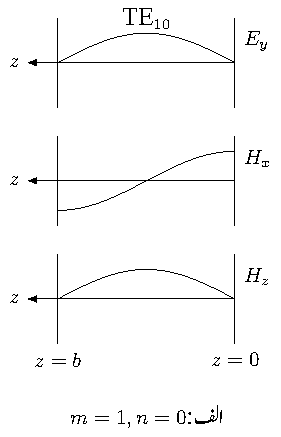
\includegraphics{figWaveguidesTE10Fields}
\end{subfigure}%
%
\begin{subfigure}{0.4\textwidth}
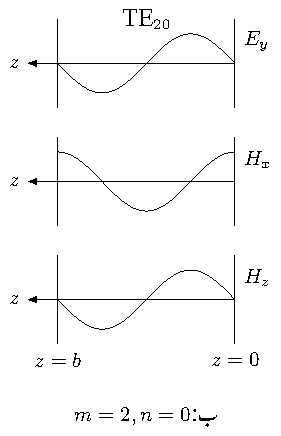
\includegraphics{figWaveguidesTE20Fields}
\end{subfigure}%
\caption{بلند  انداز \عددیء{\TE{}} امواج۔}
\label{شکل_مویج_بلند_ایک_صفر_دو_صفر}
\end{figure}

\جزوحصہ{مستطیلی مویج کے میدان پر تفصیلی غور}
%
\جزوحصہء{بلند درجی \عددیء{\TE{10}} موج:}
مساوات \حوالہ{مساوات_مویج_مکمل_الف} تا مساوات \حوالہ{مساوات_مویج_مکمل_ث} میں \عددیء{m=1} اور \عددیء{n=0} پر کرنے سے مندرجہ ذیل \عددیء{\TE{10}} امواج حاصل ہوتے ہیں۔
\begin{gather}
 \begin{aligned}
E_x&=0 \quad \quad \quad \quad \text{\RL{TE کا بنیادی شرط}}\\
E_y&=\frac{\gamma  Z_{yz} H_0}{k^2}\frac{\pi}{z_1}  \sin \frac{\pi z}{z_1} e^{j \omega t -\gamma x}\\
E_z&=0\\
H_x&=H_0   \cos  \frac{\pi z}{z_1} e^{j \omega t-\gamma x}\\
H_y&=0\\
H_z&=\frac{\gamma H_0}{k^2}\frac{\pi}{z_1}  \sin \frac{\pi z}{z_1} e^{j \omega t -\gamma x}
\end{aligned}
\end{gather}

ان میں پہلی مساوات، یعنی \عددیء{E_x=0}، درحقیقت \عددیء{\TE{}} موج کی تعریف ہے۔ان امواج کو شکل \حوالہ{شکل_مویج_بلند_ایک_صفر_دو_صفر}-الف میں \عددیء{t=0} اور \عددیء{x=0} کی صورت میں دکھایا گیا ہے۔ان اشکال میں میدان بالمقابل \عددیء{z} دکھایا گیا ہے۔مندرجہ بالا مساوات میں کوئی میدان بھی \عددیء{y} پر منحصر نہیں ہے لہٰذا \عددیء{y} کے تبدیلی سے یہ میدان تبدیل نہیں ہوں گے۔\عددیء{\TE{10}} تمام اقسام کے بلند درجی امواج میں سب سے لمبی انقطاعی طول موج رکھتی ہے لہٰذا اس کی انقطاعی تعدد سب سے کم ہے۔شکل \حوالہ{شکل_مویج_عرضی_برقی_ایک_صفر_میدان} میں \عددیء{E_y} اور \عددیء{H_z} کو بطور سمتیہ دکھایا گیا ہے۔شکل-الف میں \عددیء{z=\tfrac{z_1}{2}} پر سمتیوں کی تعداد  زیادہ دکھا کر گھنے میدان کو ظاہر کرنے کی کوشش کی گئی ہے۔ساتھ ہی ساتھ اس خطے کو گہرا رنگ بھی دے کر گھنے میدان کو ظاہر کیا گیا ہے۔شکل-ب میں مقناطیسی میدان کی سمت کو سمتیہ سے جبکہ میدان کو گہرے رنگ سے ظاہر کیا گیا ہے۔ 

\begin{figure}
\centering
\begin{subfigure}{0.4\textwidth}
\centering
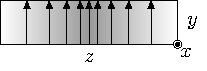
\includegraphics{figWaveguidesTE10VectorEy}
\caption*{\عددیء{\TE{10}} کا \عددیء{E_y} میدان۔}
\end{subfigure}%
%
\begin{subfigure}{0.4\textwidth}
\centering
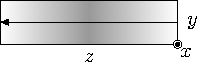
\includegraphics{figWaveguidesTE10VectorHz}
\caption*{\عددیء{\TE{10}} کا \عددیء{H_z} میدان۔}
\end{subfigure}%
\vspace{1cm}
\begin{subfigure}{0.4\textwidth}
\centering
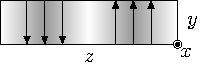
\includegraphics{figWaveguidesTE20VectorEy}
\caption*{\عددیء{\TE{20}} کا \عددیء{E_y} میدان۔}
\end{subfigure}%
%
\begin{subfigure}{0.4\textwidth}
\centering
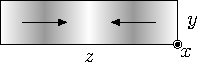
\includegraphics{figWaveguidesTE20VectorHz}
\caption*{\عددیء{\TE{20}} کا \عددیء{H_z} میدان۔}
\end{subfigure}%
\caption{\عددیء{\TE{10}} اور \عددیء{\TE{20}} کے \عددیء{E_y} اور \عددیء{H_z} میدان۔}
\label{شکل_مویج_عرضی_برقی_ایک_صفر_میدان}
\end{figure}

\جزوحصہء{بلند درجی \عددیء{\TE{20}} موج:}
شکل \حوالہ{شکل_مویج_عرضی_برقی_ایک_صفر_میدان} میں \عددیء{\TE{20}} کے \عددیء{E_y} اور \عددیء{H_z} اشکال بھی دکھائے گئے ہیں۔

\جزوحصہء{بلند درجی \عددیء{\TE{11}} موج:}
مساوات \حوالہ{مساوات_مویج_مکمل_الف} تا مساوات \حوالہ{مساوات_مویج_مکمل_ث} میں \عددیء{m=1} اور \عددیء{n=1} پر کرنے سے مندرجہ ذیل \عددیء{\TE{11}} امواج حاصل ہوتے ہیں۔
\begin{gather}
\begin{aligned}
E_x&=0 \quad \quad \quad \quad \text{\RL{TE کا بنیادی شرط}}\\
E_y&=\frac{\gamma  Z_{yz} H_0}{k^2}\frac{ \pi}{z_1} \cos \frac{\pi y}{y_1} \sin \frac{ \pi z}{z_1} e^{j \omega t -\gamma x}\\
E_z&=-\frac{\gamma  Z_{yz} H_0}{k^2}\frac{ \pi}{y_1} \sin \frac{\pi y}{y_1} \cos \frac{ \pi z}{z_1} e^{j \omega t -\gamma x}\\
H_x&=H_0 \cos \frac{ \pi y}{y_1}  \cos  \frac{ \pi z}{z_1} e^{j \omega t -\gamma x}\\
H_y&=\frac{\gamma H_0}{k^2}\frac{ \pi}{y_1} \sin \frac{\pi y}{y_1} \cos \frac{ \pi z}{z_1} e^{j \omega t -\gamma x} \\
H_z&=\frac{\gamma H_0}{k^2}\frac{ \pi}{z_1} \cos \frac{\pi y}{y_1} \sin \frac{ \pi z}{z_1} e^{j \omega t -\gamma x}
\end{aligned}
\end{gather}
%
\begin{figure}
\centering
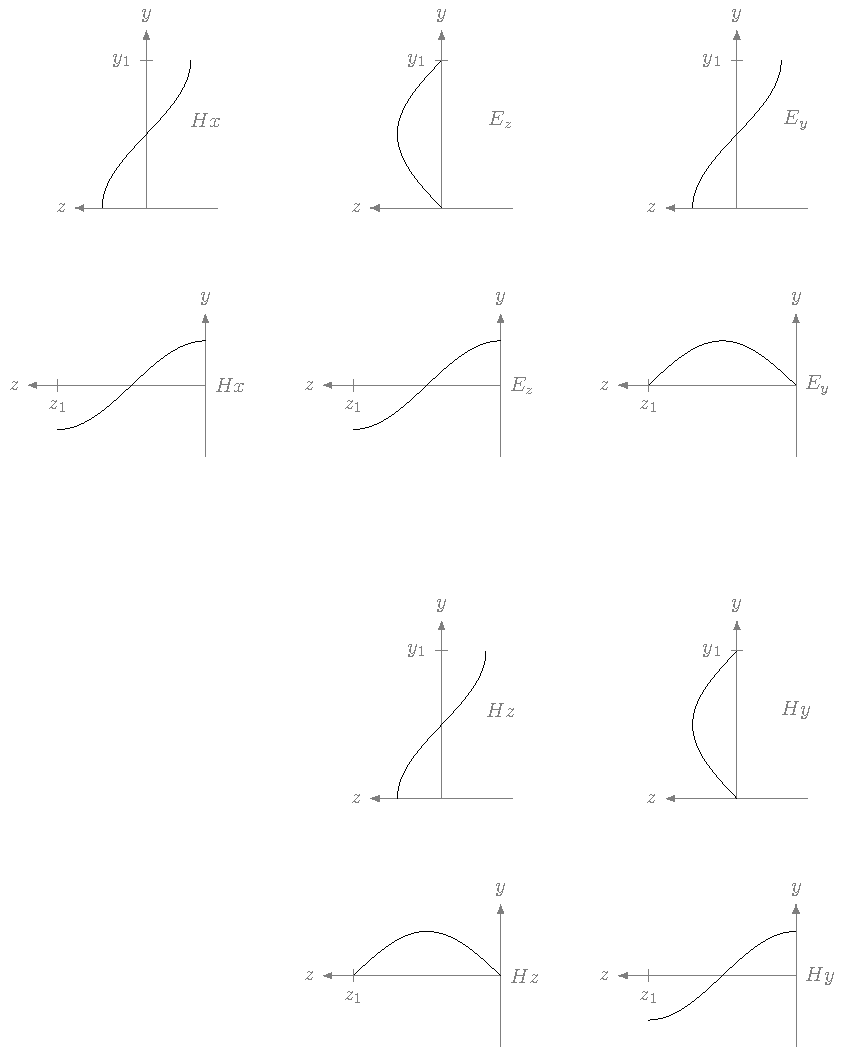
\includegraphics{figWaveguidesTE11Fields}
\caption{\عددیء{\TE{11}} میدان۔}
\label{شکل_مویج_مستطیل_ایک_ایک_برقی}
\end{figure}
اس بلند درجی انداز میں صرف \عددیء{E_x} ہر نقطے پر تمام اوقات صفر کے برابر رہتا ہے۔ان میدان کو شکل \حوالہ{شکل_مویج_مستطیل_ایک_ایک_برقی} میں دکھایا گیا ہے۔

مستطیل مویج کے حاصل حل میدان تمام ممکنہ میدان ہیں جو کسی مویج میں پائے جا سکتے ہیں۔حقیقت میں کسی بھی مویج میں پائے جانے والے امواج کا دارومدار مویج کی جسامت، موج پیدا کرنے کا طریقہ اور مویج میں نا ہمواریوں پر ہے۔کسی بھی نقطے پر موجود تمام میدانوں کا مجموعی میدان پایا جائے گا۔

واپس اپنی گفتگو پر آتے ہوئے مساوات \حوالہ{مساوات_مویج_مختلف_مستقل_تعلق}، مساوات \حوالہ{مساوات_مویج_عمومی_حل_پہلا_مستقل} اور مساوات \حوالہ{مساوات_مویج_عمومی_حل_دوسرا_مستقل} کو ملا کر
\begin{align}
k^2=\left( \frac{n \pi}{y_1}\right)^2+\left( \frac{m \pi}{z_1}\right)^2
\end{align}
لکھا جا سکتا ہے جہاں   مساوات \حوالہ{مساوت_مویج_رکاوٹ_فراوانی}، مساوات \حوالہ{مساوات_میوج_خ} اور مساوات \حوالہ{مساوات_میوج_ڑ} سے 
\begin{align}
k^2=\gamma^2-j \omega \mu (\sigma+j \omega \epsilon)
\end{align}
کے برابر ہے۔بے ضیاع ذو برق میں \عددیء{\sigma =0} لیا جا سکتا ہے۔اس طرح مندرجہ بالا دو مساوات سے
\begin{align}\label{مساوات_مویج_تعدد_بالمقابل_درجہ_انداز}
\gamma=\sqrt{\left(\frac{n\pi}{y_1}\right)^2+\left(\frac{m\pi}{z_1}\right)^2-\omega^2 \mu \epsilon}
\end{align}
حاصل ہوتا ہے۔

ایک مخصوص قیمت سے کم تعدد پر جزر میں آخری جزو پہلے دو اجزاء کے مجموعے سے کم ہو گا لہٰذا \عددیء{\gamma} حقیقی ہو گا۔حقیقی \عددیء{\gamma} کی صورت میں موج گھٹے گی اور یہ مویج میں صفر نہیں کر پائے گی۔

اسی طرح اس مخصوص قیمت سے زیادہ تعدد پر \عددیء{\gamma} خیالی عدد ہو گا لہٰذا مویج میں موج صفر کرے گی۔

ان دو قیمتوں کے درمیان تعدد کی وہ قیمت ہو گی جس پر \عددیء{\gamma=0} حاصل ہوتا ہے۔اس تعدد کو \اصطلاح{انقطاعی تعدد}\فرہنگ{انقطاعی تعدد}\فرہنگ{تعدد!انقطاعی}\حاشیہب{cutoff frequency}\فرہنگ{cutoff frequency} کہتے ہیں۔انقطاعی تعدد سے بلند تعدد کے امواج، بغیر گھٹے،  مویج میں صفر کر سکتے ہیں جبکہ اس سے کم تعدد کے امواج گھٹتے ہیں لہٰذا یہ مویج میں صفر نہیں کر پاتے۔

ان تین تعددی خطوں کو ایک جگہ دوبارہ پیش کرتے ہیں۔
\begin{itemize}
\item
کم تعدد یعنی کم \عددیء{\omega} پر \عددیء{\gamma} حقیقی ہوتا ہے۔مویج غیر شفاف ہوتا ہے جس میں امواج صفر نہیں کر سکتے۔
\item
مخصوص درمیانی تعدد پر \عددیء{\gamma=0} ہوتا ہے۔یہ انقطاعی تعدد ہے۔
\item
زیادہ تعدد پر \عددیء{\gamma} خیالی ہوتا ہے۔مویج شفاف ہوتا ہے جس میں امواج صفر کر سکتے ہیں۔
\end{itemize}

مساوات \حوالہ{مساوات_مویج_تعدد_بالمقابل_درجہ_انداز} میں \عددیء{\sqrt{\omega^2 \mu \epsilon}} درحقیقت ایسی لامحدود خطے کا زاویائی مستقل \عددیء{\beta_0} ہے جس میں وہی ذو برق ہو جو مویج میں پایا جاتا ہے۔یوں ہم
\begin{align}
\gamma=\sqrt{k^2-\beta_0^2}
\end{align}
لکھ سکتے ہیں جہاں
\begin{align*}
\beta_0&=\sqrt{\omega^2 \mu \epsilon}=\frac{2\pi}{\lambda_0} \quad \text{\RL{لامحدود خطے کا زاویائی مستقل}}\\
\lambda_0 & \quad \text{\RL{لامحدود خطے میں طول موج}}\\
k&=\sqrt{\left(\frac{n\pi}{y_1}\right)^2+\left(\frac{m\pi}{z_1}\right)^2}
\end{align*}
ہیں۔یوں انقطاعی تعدد سے بلند تعدد پر \عددیء{\beta_0 > k} ہو گا لہٰذا
\begin{align}
\gamma=\sqrt{k^2-\beta_0^2}=j\beta
\end{align}
ہو گا جہاں
\begin{align*}
\beta&=\frac{2\pi}{\lambda}=\sqrt{\beta_0^2-k^2} \quad{\text{\RL{مویج میں زاویائی مستقل}}} \\
\lambda& \quad \text{\RL{مویج میں طول موج}}
\end{align*}
ہیں۔کافی بلند تعدد پر \عددیء{\beta_0 \gg k} ہو گا اور یوں مویج کے زاویائی مستقل \عددیء{\beta} کی قیمت لامحدود خطے کے زاویائی مستقل \عددیء{\beta_0} کے قیمت کے قریب ہو گی۔اس کے برعکس انقطاعی تعدد سے کم تعدد پر \عددیء{\beta_0 < k} ہو گا جس سے
\begin{align}
\gamma=\sqrt{k^2-\beta_0^2}=\alpha
\end{align}
حاصل ہوتا ہے جہاں \عددیء{\alpha} تقلیلی مستقل ہے۔

کافی کم تعدد پر \عددیء{\beta_0 \ll k} ہو گا لہٰذا تقلیلی مستقل کی قیمت  \عددیء{k}  کے قریب ہو گی۔

عین انقطاعی تعدد پر \عددیء{\beta_0=k} ہو گا لہٰذا \عددیء{\gamma=0} ہو گا۔یوں انقطاعی تعدد پر
\begin{align}
\omega^2 \mu \epsilon =\left(\frac{n\pi}{y_1}\right)^2+\left(\frac{m\pi}{z_1}\right)^2
\end{align}
ہو گا جس سے \اصطلاح{انقطاعی تعدد}\فرہنگ{انقطاعی!تعدد}\حاشیہب{cutoff frequency}\فرہنگ{cutoff!frequency}
\begin{align}\label{مساوات_مویج_مستطیلی-انقطاعی_تعدد}
f_c=\frac{1}{2 \sqrt{\mu \epsilon}} \sqrt{\left(\frac{n}{y_1}\right)^2+\left(\frac{m}{z_1}\right)^2} \quad \quad (\si{\hertz})
\end{align}
اور انقطاعی طول موج
\begin{align}\label{مساوات_مویج_مستطیلی-انقطاعی_طول_موج}
\lambda_{0c}=\frac{2\pi}{\sqrt{\left(\frac{n\pi}{y_1}\right)^2+\left(\frac{m\pi}{z_1}\right)^2}}=\frac{2}{\sqrt{\left(\frac{n}{y_1}\right)^2+\left(\frac{m}{z_1}\right)^2}}=\frac{2\pi}{k}  \quad \quad (\si{\meter})
\end{align}
حاصل ہوتے ہیں جہاں \عددیء{\lambda_{0c}} لامحدود خطے میں انقطاعی تعدد پر طول موج ہے جسے چھوٹا کر کہ \اصطلاح{انقطاعی طول موج}\فرہنگ{انقطاعی!طول موج}\حاشیہب{cutoff wavelength}\فرہنگ{cutoff!wavelength} پکارا جاتا ہے۔مساوات \حوالہ{مساوات_مویج_مستطیلی-انقطاعی_تعدد} اور مساوات \حوالہ{مساوات_مویج_مستطیلی-انقطاعی_طول_موج} سے کھوکھلے مستطیلی مویج کے کسی بھی \عددیء{\TE{mn}} موج کا انقطاعی تعدد اور انقطاعی طول موج حاصل کیا جا سکتا ہے۔مثال کے
 طور پر \عددیء{\TE{10}} موج کا انقطاعی طول موج
\begin{align}
\lambda_{0c}=2 z_1
\end{align}
حاصل ہوتا ہے جو وہی قیمت ہے جو مساوات \حوالہ{مساوات_مویج_دو_چادر_انقطاعی_طول_موج} میں حاصل کی گئی تھی جہاں \عددیء{z_1=b} کے برابر ہے۔ 

انقطاعی تعدد سے بلند تعدد \عددیء{(\beta_0 > k)}  پر
\begin{align}
\beta=\sqrt{\beta_0^2-k^2}=\sqrt{\omega^2 \mu \epsilon -\left(\frac{n \pi}{y_1}\right)^2-\left(\frac{m \pi}{z_1}\right)^2}
\end{align}
لہٰذا  مویج میں \اصطلاح{دوری رفتار}\فرہنگ{دوری!رفتار}\فرہنگ{رفتار!دوری}\حاشیہب{phase velocity}\فرہنگ{phase!velocity} \عددیء{v_p}
\begin{align}
v_p =\frac{\omega}{\beta}=\frac{v_0}{\sqrt{1-\left(\frac{n \lambda_0}{2 y_1}\right)^2-\left(\frac{m \lambda_0}{2 z_1}\right)^2}}
\end{align}
یا
\begin{align}
v_p=\frac{v_0}{\sqrt{1-\left(\frac{\lambda_0}{\lambda_{0c}}\right)^2}}
\end{align}
ہو گی جہاں
\begin{align*}
v_0&=\frac{1}{\sqrt{\mu \epsilon}} \quad \quad \text{\RL{لامحدود خطے میں دوری رفتار}} \\
\lambda_0& \quad \quad \text{\RL{لامحدود خطے میں طول موج}}\\
\lambda_{0c}& \quad \quad \text{\RL{ انقطاعی طول موج}}
\end{align*}
ہیں۔
\begin{figure}
\centering
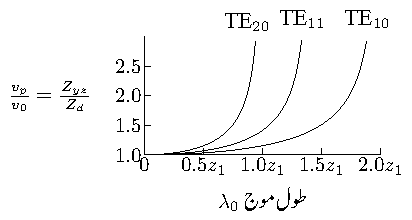
\includegraphics{figWaveguidesVelocityVersusMode}
\caption{مختلف بلند درجی امواج کے مستطیلی مویج میں دوری رفتار بالمقابل طول موج \عددیء{\lambda_0}۔}
\label{شکل_مویج_دوری_رفتار_مختلف_بلند_انداز}
\end{figure}

شکل \حوالہ{شکل_مویج_دوری_رفتار_مختلف_بلند_انداز} میں مختلف بلند انداز امواج  کے دوری رفتار بالمقابل طول موج \عددیء{\lambda_0} دکھائے گئے ہیں۔دوری رفتار کو لامحدود خطے کے دوری رفتار  \عددیء{v_0} کی نسبت سے دکھایا گیا ہے۔ان اشکال میں مستطیلی مویج کے دونوں اطراف برابر لمبائی \عددیء{(y_1=z_1)} کے تصور کئے گئے ہیں۔

مندرجہ بالا تجزیے میں مویج کے اطراف کامل موصل کے تصور کئے گئے اور ساتھ ہی ساتھ مویج میں بے ضیاع ذو برق بھرا تصور کیا گیا۔اسی لئے انقطاعی تعدد سے بلند تعدد پر امواج بغیر گھٹے مویج میں صفر کرتے ہیں۔حقیقت میں مویج کے اطراف کے موصل کی موصلیت اور ذو برق میں طاقت کی ضیاع سے \عددیء{\gamma=\alpha+j\beta}  ہو گا لہٰذا انقطاعی تعدد سے بلند تعدد کے امواج بھی صفر کے دوران کچھ نہ کچھ گھٹتے ہیں۔

کھوکھلے مویج جس میں صرف ہوا بھری ہو میں ذو برق یعنی ہوا کا ضیاع  قابل نظر انداز ہوتا ہے۔ایسے مویج میں طاقت کا ضیاع صرف مویج کے چادروں کی موصلیت کی بنا ہے۔موصل چادر مکمل طور پر کامل نہ ہونے کا مطلب لے کہ حقیقت میں چادر کے متوازی برقی میدان \عددیء{E_m} صفر نہیں ہو گا۔اچھے موصل مثلاً تانبے کی بنی چادر میں \عددیء{E_m} کی قیمت قابل نظر انداز ہوتی ہے۔یوں تانبے یا دیگر اچھے موصل کے چادر سے بنی مویج کے طول موج \عددیء{\lambda}، زاویائی مستقل \عددیء{\beta} یا دوری رفتار \عددیء{v_p} حاصل کرتے وقت مویج کے چادر کو کامل ہی تصور کیا جاتا ہے۔ایسی صورت میں تقلیلی مستقل \عددیء{\alpha} کا تخمینہ  علیحدہ طور پر لگایا جاتا ہے۔

آخر میں مستطیلی مویج میں عرضی برقی موج کی رکاوٹ \عددیء{Z_{yz}} مساوات \حوالہ{مساوات_میوج_خ} سے حاصل کرتے ہیں۔
\begin{align}
Z_{yz}=\frac{j\omega \mu}{\gamma}
\end{align} 
انقطاعی تعدد سے بلند تعدد پر \عددیء{\gamma=j\beta} ہوتا ہے لہٰذا
\begin{align*}
Z_{yz}=\frac{\omega \mu}{\beta}=\frac{Z_d}{\sqrt{1-\left(\frac{\lambda_0}{\lambda_{0c}}\right)^2}} \quad \quad (\si{\ohm})
\end{align*} 
ہو گا جہاں
\begin{align*}
Z_d&=\sqrt{\frac{\mu}{\epsilon}} \quad \text{\RL{مویج کے ذو برق کی قدرتی رکاوٹ}} \\
\lambda_0& \quad \text{\RL{لامحدود خطے میں طول موج}}\\
\lambda_{0c}& \quad \text{\RL{انقطاعی طول موج}}
\end{align*}
ہیں۔ہوا کے لئے \عددیء{Z_d=120 \pi=\SI{376.7}{\ohm}} کے برابر ہے۔چونکہ \عددیء{Z_{yz}} اور \عددیء{Z_d} کی شرح بالقل \عددیء{v_p} اور \عددیء{v_0} کی شرح کے برابر ہے لہٰذا شکل  \حوالہ{شکل_مویج_دوری_رفتار_مختلف_بلند_انداز} \عددیء{\tfrac{Z_{yz}}{Z_d}} بالمقابل \عددیء{\lambda_0} بھی دیتا ہے۔


\حصہ{مستطیلی مویج میں عرضی مقناطیسی \عددیء{\TM{mn}} موج}
عرضی برقی امواج حل کرنے کے آٹھ اقدام صفحہ \حوالہصفحہ{اقدام_مویج_آٹھ_قدم} پر بتلائے گئے۔انہیں آٹھ قدم سے عرضی مقناطیسی موج بھی حاصل کئے جاتے ہیں۔ باب کے آخر میں آپ کو یہی راہ استعمال کرتے ہوئے، مستطیلی مویج میں  \عددیء{\TM{mn}} موج  حاصل کرنے کو کہا گیا ہے۔آئیں یہاں مستطیلی  مویج میں \عددیء{\TM{mn}} موج حاصل کرنے کا ذرہ گہرا طریقہ استعمال کریں۔

چارج سے خالی خلاء \عددیء{(\rho_h=0)} کی صورت میں میں میکس ویل کے مساوات
\begin{align*}
\nabla \times \kvec{E}&=-\frac{\partial \kvec{B}}{\partial t}=-\mu \frac{\partial \kvec{H}}{\partial t}\\
\nabla \times \kvec{H}&=\kvec{J}_d+\frac{\partial \kvec{D}}{\partial t}=\sigma \kvec{E}+\epsilon \frac{\partial \kvec{E}}{\partial t}\\
\nabla \cdot \kvec{E}&=0\\
\nabla \cdot \kvec{H}&=0
\end{align*}
میں وقت کے ساتھ سائن نما تعلق اور فاصلے کے ساتھ سائن نما تعلق کا شرط یعنی مساوات \حوالہ{مساوات_مویج_سائن_نما_کی_قید} لاگو کرنے سے 
\begin{gather}
\begin{aligned}\label{مساوات_مویج_مقناطیسی_الف}
\nabla \times \kvec{E}&=-j \omega \mu \kvec{H} =Z \kvec{H}\\
\nabla \times \kvec{H}&=\sigma \kvec{E}+j \omega \epsilon  \kvec{E}=Y \kvec{E}\\
\nabla \cdot \kvec{E}&=0\\
\nabla \cdot \kvec{H}&=0
\end{aligned}
\end{gather}
حاصل ہوتا ہے جہاں مساوات \حوالہ{مساوت_مویج_رکاوٹ_فراوانی} کا استعمال کیا گیا۔ان میں دوسری مساوات کی گردش لے کر پہلا مساوات پر کرتے ہوئے
\begin{align*}
\nabla \times \nabla \times \kvec{H}&=Y \nabla \times \kvec{E}=Y Z\kvec{H}
\end{align*}
لکھا جا سکتا ہے جسے مزید یوں
\begin{align*}
\nabla \left(\nabla \cdot \kvec{H} \right)-\nabla^2 \kvec{H}=YZ\kvec{H}
\end{align*}
لکھا جا سکتا ہے۔مساوات \حوالہ{مساوات_مویج_مقناطیسی_الف} کے تحت \عددیء{\nabla \cdot \kvec{H}=0} ہے لہٰذا
\begin{align*}
\nabla^2 \kvec{H}+YZ\kvec{H}=0
\end{align*}
حاصل ہوتا ہے۔یہ مساوات درحقیقت تین مختلف مساوات کو ظاہر کرتی ہے۔اس کا \عددیء{H_x} جزو
\begin{align*}
\nabla^2 H_x+YZ H_x=0
\end{align*}
یعنی
\begin{align*}
\frac{\partial^2 H_x}{\partial x^2}+\frac{\partial^2 H_x}{\partial y^2}+\frac{\partial^2 H_x}{\partial z^2}+YZ H_x=0
\end{align*}
ہے۔
